
% Default to the notebook output style

    


% Inherit from the specified cell style.




    
\documentclass[11pt]{article}

    
    
    \usepackage[T1]{fontenc}
    % Nicer default font (+ math font) than Computer Modern for most use cases
    \usepackage{mathpazo}

    % Basic figure setup, for now with no caption control since it's done
    % automatically by Pandoc (which extracts ![](path) syntax from Markdown).
    \usepackage{graphicx}
    % We will generate all images so they have a width \maxwidth. This means
    % that they will get their normal width if they fit onto the page, but
    % are scaled down if they would overflow the margins.
    \makeatletter
    \def\maxwidth{\ifdim\Gin@nat@width>\linewidth\linewidth
    \else\Gin@nat@width\fi}
    \makeatother
    \let\Oldincludegraphics\includegraphics
    % Set max figure width to be 80% of text width, for now hardcoded.
    \renewcommand{\includegraphics}[1]{\Oldincludegraphics[width=.8\maxwidth]{#1}}
    % Ensure that by default, figures have no caption (until we provide a
    % proper Figure object with a Caption API and a way to capture that
    % in the conversion process - todo).
    \usepackage{caption}
    \DeclareCaptionLabelFormat{nolabel}{}
    \captionsetup{labelformat=nolabel}

    \usepackage{adjustbox} % Used to constrain images to a maximum size 
    \usepackage{xcolor} % Allow colors to be defined
    \usepackage{enumerate} % Needed for markdown enumerations to work
    \usepackage{geometry} % Used to adjust the document margins
    \usepackage{amsmath} % Equations
    \usepackage{amssymb} % Equations
    \usepackage{textcomp} % defines textquotesingle
    % Hack from http://tex.stackexchange.com/a/47451/13684:
    \AtBeginDocument{%
        \def\PYZsq{\textquotesingle}% Upright quotes in Pygmentized code
    }
    \usepackage{upquote} % Upright quotes for verbatim code
    \usepackage{eurosym} % defines \euro
    \usepackage[mathletters]{ucs} % Extended unicode (utf-8) support
    \usepackage[utf8x]{inputenc} % Allow utf-8 characters in the tex document
    \usepackage{fancyvrb} % verbatim replacement that allows latex
    \usepackage{grffile} % extends the file name processing of package graphics 
                         % to support a larger range 
    % The hyperref package gives us a pdf with properly built
    % internal navigation ('pdf bookmarks' for the table of contents,
    % internal cross-reference links, web links for URLs, etc.)
    \usepackage{hyperref}
    \usepackage{longtable} % longtable support required by pandoc >1.10
    \usepackage{booktabs}  % table support for pandoc > 1.12.2
    \usepackage[inline]{enumitem} % IRkernel/repr support (it uses the enumerate* environment)
    \usepackage[normalem]{ulem} % ulem is needed to support strikethroughs (\sout)
                                % normalem makes italics be italics, not underlines
    

    
    
    % Colors for the hyperref package
    \definecolor{urlcolor}{rgb}{0,.145,.698}
    \definecolor{linkcolor}{rgb}{.71,0.21,0.01}
    \definecolor{citecolor}{rgb}{.12,.54,.11}

    % ANSI colors
    \definecolor{ansi-black}{HTML}{3E424D}
    \definecolor{ansi-black-intense}{HTML}{282C36}
    \definecolor{ansi-red}{HTML}{E75C58}
    \definecolor{ansi-red-intense}{HTML}{B22B31}
    \definecolor{ansi-green}{HTML}{00A250}
    \definecolor{ansi-green-intense}{HTML}{007427}
    \definecolor{ansi-yellow}{HTML}{DDB62B}
    \definecolor{ansi-yellow-intense}{HTML}{B27D12}
    \definecolor{ansi-blue}{HTML}{208FFB}
    \definecolor{ansi-blue-intense}{HTML}{0065CA}
    \definecolor{ansi-magenta}{HTML}{D160C4}
    \definecolor{ansi-magenta-intense}{HTML}{A03196}
    \definecolor{ansi-cyan}{HTML}{60C6C8}
    \definecolor{ansi-cyan-intense}{HTML}{258F8F}
    \definecolor{ansi-white}{HTML}{C5C1B4}
    \definecolor{ansi-white-intense}{HTML}{A1A6B2}

    % commands and environments needed by pandoc snippets
    % extracted from the output of `pandoc -s`
    \providecommand{\tightlist}{%
      \setlength{\itemsep}{0pt}\setlength{\parskip}{0pt}}
    \DefineVerbatimEnvironment{Highlighting}{Verbatim}{commandchars=\\\{\}}
    % Add ',fontsize=\small' for more characters per line
    \newenvironment{Shaded}{}{}
    \newcommand{\KeywordTok}[1]{\textcolor[rgb]{0.00,0.44,0.13}{\textbf{{#1}}}}
    \newcommand{\DataTypeTok}[1]{\textcolor[rgb]{0.56,0.13,0.00}{{#1}}}
    \newcommand{\DecValTok}[1]{\textcolor[rgb]{0.25,0.63,0.44}{{#1}}}
    \newcommand{\BaseNTok}[1]{\textcolor[rgb]{0.25,0.63,0.44}{{#1}}}
    \newcommand{\FloatTok}[1]{\textcolor[rgb]{0.25,0.63,0.44}{{#1}}}
    \newcommand{\CharTok}[1]{\textcolor[rgb]{0.25,0.44,0.63}{{#1}}}
    \newcommand{\StringTok}[1]{\textcolor[rgb]{0.25,0.44,0.63}{{#1}}}
    \newcommand{\CommentTok}[1]{\textcolor[rgb]{0.38,0.63,0.69}{\textit{{#1}}}}
    \newcommand{\OtherTok}[1]{\textcolor[rgb]{0.00,0.44,0.13}{{#1}}}
    \newcommand{\AlertTok}[1]{\textcolor[rgb]{1.00,0.00,0.00}{\textbf{{#1}}}}
    \newcommand{\FunctionTok}[1]{\textcolor[rgb]{0.02,0.16,0.49}{{#1}}}
    \newcommand{\RegionMarkerTok}[1]{{#1}}
    \newcommand{\ErrorTok}[1]{\textcolor[rgb]{1.00,0.00,0.00}{\textbf{{#1}}}}
    \newcommand{\NormalTok}[1]{{#1}}
    
    % Additional commands for more recent versions of Pandoc
    \newcommand{\ConstantTok}[1]{\textcolor[rgb]{0.53,0.00,0.00}{{#1}}}
    \newcommand{\SpecialCharTok}[1]{\textcolor[rgb]{0.25,0.44,0.63}{{#1}}}
    \newcommand{\VerbatimStringTok}[1]{\textcolor[rgb]{0.25,0.44,0.63}{{#1}}}
    \newcommand{\SpecialStringTok}[1]{\textcolor[rgb]{0.73,0.40,0.53}{{#1}}}
    \newcommand{\ImportTok}[1]{{#1}}
    \newcommand{\DocumentationTok}[1]{\textcolor[rgb]{0.73,0.13,0.13}{\textit{{#1}}}}
    \newcommand{\AnnotationTok}[1]{\textcolor[rgb]{0.38,0.63,0.69}{\textbf{\textit{{#1}}}}}
    \newcommand{\CommentVarTok}[1]{\textcolor[rgb]{0.38,0.63,0.69}{\textbf{\textit{{#1}}}}}
    \newcommand{\VariableTok}[1]{\textcolor[rgb]{0.10,0.09,0.49}{{#1}}}
    \newcommand{\ControlFlowTok}[1]{\textcolor[rgb]{0.00,0.44,0.13}{\textbf{{#1}}}}
    \newcommand{\OperatorTok}[1]{\textcolor[rgb]{0.40,0.40,0.40}{{#1}}}
    \newcommand{\BuiltInTok}[1]{{#1}}
    \newcommand{\ExtensionTok}[1]{{#1}}
    \newcommand{\PreprocessorTok}[1]{\textcolor[rgb]{0.74,0.48,0.00}{{#1}}}
    \newcommand{\AttributeTok}[1]{\textcolor[rgb]{0.49,0.56,0.16}{{#1}}}
    \newcommand{\InformationTok}[1]{\textcolor[rgb]{0.38,0.63,0.69}{\textbf{\textit{{#1}}}}}
    \newcommand{\WarningTok}[1]{\textcolor[rgb]{0.38,0.63,0.69}{\textbf{\textit{{#1}}}}}
    
    
    % Define a nice break command that doesn't care if a line doesn't already
    % exist.
    \def\br{\hspace*{\fill} \\* }
    % Math Jax compatability definitions
    \def\gt{>}
    \def\lt{<}
    % Document parameters
    \title{Linear Algebra Introduction}
    
    
    

    % Pygments definitions
    
\makeatletter
\def\PY@reset{\let\PY@it=\relax \let\PY@bf=\relax%
    \let\PY@ul=\relax \let\PY@tc=\relax%
    \let\PY@bc=\relax \let\PY@ff=\relax}
\def\PY@tok#1{\csname PY@tok@#1\endcsname}
\def\PY@toks#1+{\ifx\relax#1\empty\else%
    \PY@tok{#1}\expandafter\PY@toks\fi}
\def\PY@do#1{\PY@bc{\PY@tc{\PY@ul{%
    \PY@it{\PY@bf{\PY@ff{#1}}}}}}}
\def\PY#1#2{\PY@reset\PY@toks#1+\relax+\PY@do{#2}}

\expandafter\def\csname PY@tok@w\endcsname{\def\PY@tc##1{\textcolor[rgb]{0.73,0.73,0.73}{##1}}}
\expandafter\def\csname PY@tok@c\endcsname{\let\PY@it=\textit\def\PY@tc##1{\textcolor[rgb]{0.25,0.50,0.50}{##1}}}
\expandafter\def\csname PY@tok@cp\endcsname{\def\PY@tc##1{\textcolor[rgb]{0.74,0.48,0.00}{##1}}}
\expandafter\def\csname PY@tok@k\endcsname{\let\PY@bf=\textbf\def\PY@tc##1{\textcolor[rgb]{0.00,0.50,0.00}{##1}}}
\expandafter\def\csname PY@tok@kp\endcsname{\def\PY@tc##1{\textcolor[rgb]{0.00,0.50,0.00}{##1}}}
\expandafter\def\csname PY@tok@kt\endcsname{\def\PY@tc##1{\textcolor[rgb]{0.69,0.00,0.25}{##1}}}
\expandafter\def\csname PY@tok@o\endcsname{\def\PY@tc##1{\textcolor[rgb]{0.40,0.40,0.40}{##1}}}
\expandafter\def\csname PY@tok@ow\endcsname{\let\PY@bf=\textbf\def\PY@tc##1{\textcolor[rgb]{0.67,0.13,1.00}{##1}}}
\expandafter\def\csname PY@tok@nb\endcsname{\def\PY@tc##1{\textcolor[rgb]{0.00,0.50,0.00}{##1}}}
\expandafter\def\csname PY@tok@nf\endcsname{\def\PY@tc##1{\textcolor[rgb]{0.00,0.00,1.00}{##1}}}
\expandafter\def\csname PY@tok@nc\endcsname{\let\PY@bf=\textbf\def\PY@tc##1{\textcolor[rgb]{0.00,0.00,1.00}{##1}}}
\expandafter\def\csname PY@tok@nn\endcsname{\let\PY@bf=\textbf\def\PY@tc##1{\textcolor[rgb]{0.00,0.00,1.00}{##1}}}
\expandafter\def\csname PY@tok@ne\endcsname{\let\PY@bf=\textbf\def\PY@tc##1{\textcolor[rgb]{0.82,0.25,0.23}{##1}}}
\expandafter\def\csname PY@tok@nv\endcsname{\def\PY@tc##1{\textcolor[rgb]{0.10,0.09,0.49}{##1}}}
\expandafter\def\csname PY@tok@no\endcsname{\def\PY@tc##1{\textcolor[rgb]{0.53,0.00,0.00}{##1}}}
\expandafter\def\csname PY@tok@nl\endcsname{\def\PY@tc##1{\textcolor[rgb]{0.63,0.63,0.00}{##1}}}
\expandafter\def\csname PY@tok@ni\endcsname{\let\PY@bf=\textbf\def\PY@tc##1{\textcolor[rgb]{0.60,0.60,0.60}{##1}}}
\expandafter\def\csname PY@tok@na\endcsname{\def\PY@tc##1{\textcolor[rgb]{0.49,0.56,0.16}{##1}}}
\expandafter\def\csname PY@tok@nt\endcsname{\let\PY@bf=\textbf\def\PY@tc##1{\textcolor[rgb]{0.00,0.50,0.00}{##1}}}
\expandafter\def\csname PY@tok@nd\endcsname{\def\PY@tc##1{\textcolor[rgb]{0.67,0.13,1.00}{##1}}}
\expandafter\def\csname PY@tok@s\endcsname{\def\PY@tc##1{\textcolor[rgb]{0.73,0.13,0.13}{##1}}}
\expandafter\def\csname PY@tok@sd\endcsname{\let\PY@it=\textit\def\PY@tc##1{\textcolor[rgb]{0.73,0.13,0.13}{##1}}}
\expandafter\def\csname PY@tok@si\endcsname{\let\PY@bf=\textbf\def\PY@tc##1{\textcolor[rgb]{0.73,0.40,0.53}{##1}}}
\expandafter\def\csname PY@tok@se\endcsname{\let\PY@bf=\textbf\def\PY@tc##1{\textcolor[rgb]{0.73,0.40,0.13}{##1}}}
\expandafter\def\csname PY@tok@sr\endcsname{\def\PY@tc##1{\textcolor[rgb]{0.73,0.40,0.53}{##1}}}
\expandafter\def\csname PY@tok@ss\endcsname{\def\PY@tc##1{\textcolor[rgb]{0.10,0.09,0.49}{##1}}}
\expandafter\def\csname PY@tok@sx\endcsname{\def\PY@tc##1{\textcolor[rgb]{0.00,0.50,0.00}{##1}}}
\expandafter\def\csname PY@tok@m\endcsname{\def\PY@tc##1{\textcolor[rgb]{0.40,0.40,0.40}{##1}}}
\expandafter\def\csname PY@tok@gh\endcsname{\let\PY@bf=\textbf\def\PY@tc##1{\textcolor[rgb]{0.00,0.00,0.50}{##1}}}
\expandafter\def\csname PY@tok@gu\endcsname{\let\PY@bf=\textbf\def\PY@tc##1{\textcolor[rgb]{0.50,0.00,0.50}{##1}}}
\expandafter\def\csname PY@tok@gd\endcsname{\def\PY@tc##1{\textcolor[rgb]{0.63,0.00,0.00}{##1}}}
\expandafter\def\csname PY@tok@gi\endcsname{\def\PY@tc##1{\textcolor[rgb]{0.00,0.63,0.00}{##1}}}
\expandafter\def\csname PY@tok@gr\endcsname{\def\PY@tc##1{\textcolor[rgb]{1.00,0.00,0.00}{##1}}}
\expandafter\def\csname PY@tok@ge\endcsname{\let\PY@it=\textit}
\expandafter\def\csname PY@tok@gs\endcsname{\let\PY@bf=\textbf}
\expandafter\def\csname PY@tok@gp\endcsname{\let\PY@bf=\textbf\def\PY@tc##1{\textcolor[rgb]{0.00,0.00,0.50}{##1}}}
\expandafter\def\csname PY@tok@go\endcsname{\def\PY@tc##1{\textcolor[rgb]{0.53,0.53,0.53}{##1}}}
\expandafter\def\csname PY@tok@gt\endcsname{\def\PY@tc##1{\textcolor[rgb]{0.00,0.27,0.87}{##1}}}
\expandafter\def\csname PY@tok@err\endcsname{\def\PY@bc##1{\setlength{\fboxsep}{0pt}\fcolorbox[rgb]{1.00,0.00,0.00}{1,1,1}{\strut ##1}}}
\expandafter\def\csname PY@tok@kc\endcsname{\let\PY@bf=\textbf\def\PY@tc##1{\textcolor[rgb]{0.00,0.50,0.00}{##1}}}
\expandafter\def\csname PY@tok@kd\endcsname{\let\PY@bf=\textbf\def\PY@tc##1{\textcolor[rgb]{0.00,0.50,0.00}{##1}}}
\expandafter\def\csname PY@tok@kn\endcsname{\let\PY@bf=\textbf\def\PY@tc##1{\textcolor[rgb]{0.00,0.50,0.00}{##1}}}
\expandafter\def\csname PY@tok@kr\endcsname{\let\PY@bf=\textbf\def\PY@tc##1{\textcolor[rgb]{0.00,0.50,0.00}{##1}}}
\expandafter\def\csname PY@tok@bp\endcsname{\def\PY@tc##1{\textcolor[rgb]{0.00,0.50,0.00}{##1}}}
\expandafter\def\csname PY@tok@fm\endcsname{\def\PY@tc##1{\textcolor[rgb]{0.00,0.00,1.00}{##1}}}
\expandafter\def\csname PY@tok@vc\endcsname{\def\PY@tc##1{\textcolor[rgb]{0.10,0.09,0.49}{##1}}}
\expandafter\def\csname PY@tok@vg\endcsname{\def\PY@tc##1{\textcolor[rgb]{0.10,0.09,0.49}{##1}}}
\expandafter\def\csname PY@tok@vi\endcsname{\def\PY@tc##1{\textcolor[rgb]{0.10,0.09,0.49}{##1}}}
\expandafter\def\csname PY@tok@vm\endcsname{\def\PY@tc##1{\textcolor[rgb]{0.10,0.09,0.49}{##1}}}
\expandafter\def\csname PY@tok@sa\endcsname{\def\PY@tc##1{\textcolor[rgb]{0.73,0.13,0.13}{##1}}}
\expandafter\def\csname PY@tok@sb\endcsname{\def\PY@tc##1{\textcolor[rgb]{0.73,0.13,0.13}{##1}}}
\expandafter\def\csname PY@tok@sc\endcsname{\def\PY@tc##1{\textcolor[rgb]{0.73,0.13,0.13}{##1}}}
\expandafter\def\csname PY@tok@dl\endcsname{\def\PY@tc##1{\textcolor[rgb]{0.73,0.13,0.13}{##1}}}
\expandafter\def\csname PY@tok@s2\endcsname{\def\PY@tc##1{\textcolor[rgb]{0.73,0.13,0.13}{##1}}}
\expandafter\def\csname PY@tok@sh\endcsname{\def\PY@tc##1{\textcolor[rgb]{0.73,0.13,0.13}{##1}}}
\expandafter\def\csname PY@tok@s1\endcsname{\def\PY@tc##1{\textcolor[rgb]{0.73,0.13,0.13}{##1}}}
\expandafter\def\csname PY@tok@mb\endcsname{\def\PY@tc##1{\textcolor[rgb]{0.40,0.40,0.40}{##1}}}
\expandafter\def\csname PY@tok@mf\endcsname{\def\PY@tc##1{\textcolor[rgb]{0.40,0.40,0.40}{##1}}}
\expandafter\def\csname PY@tok@mh\endcsname{\def\PY@tc##1{\textcolor[rgb]{0.40,0.40,0.40}{##1}}}
\expandafter\def\csname PY@tok@mi\endcsname{\def\PY@tc##1{\textcolor[rgb]{0.40,0.40,0.40}{##1}}}
\expandafter\def\csname PY@tok@il\endcsname{\def\PY@tc##1{\textcolor[rgb]{0.40,0.40,0.40}{##1}}}
\expandafter\def\csname PY@tok@mo\endcsname{\def\PY@tc##1{\textcolor[rgb]{0.40,0.40,0.40}{##1}}}
\expandafter\def\csname PY@tok@ch\endcsname{\let\PY@it=\textit\def\PY@tc##1{\textcolor[rgb]{0.25,0.50,0.50}{##1}}}
\expandafter\def\csname PY@tok@cm\endcsname{\let\PY@it=\textit\def\PY@tc##1{\textcolor[rgb]{0.25,0.50,0.50}{##1}}}
\expandafter\def\csname PY@tok@cpf\endcsname{\let\PY@it=\textit\def\PY@tc##1{\textcolor[rgb]{0.25,0.50,0.50}{##1}}}
\expandafter\def\csname PY@tok@c1\endcsname{\let\PY@it=\textit\def\PY@tc##1{\textcolor[rgb]{0.25,0.50,0.50}{##1}}}
\expandafter\def\csname PY@tok@cs\endcsname{\let\PY@it=\textit\def\PY@tc##1{\textcolor[rgb]{0.25,0.50,0.50}{##1}}}

\def\PYZbs{\char`\\}
\def\PYZus{\char`\_}
\def\PYZob{\char`\{}
\def\PYZcb{\char`\}}
\def\PYZca{\char`\^}
\def\PYZam{\char`\&}
\def\PYZlt{\char`\<}
\def\PYZgt{\char`\>}
\def\PYZsh{\char`\#}
\def\PYZpc{\char`\%}
\def\PYZdl{\char`\$}
\def\PYZhy{\char`\-}
\def\PYZsq{\char`\'}
\def\PYZdq{\char`\"}
\def\PYZti{\char`\~}
% for compatibility with earlier versions
\def\PYZat{@}
\def\PYZlb{[}
\def\PYZrb{]}
\makeatother


    % Exact colors from NB
    \definecolor{incolor}{rgb}{0.0, 0.0, 0.5}
    \definecolor{outcolor}{rgb}{0.545, 0.0, 0.0}



    
    % Prevent overflowing lines due to hard-to-break entities
    \sloppy 
    % Setup hyperref package
    \hypersetup{
      breaklinks=true,  % so long urls are correctly broken across lines
      colorlinks=true,
      urlcolor=urlcolor,
      linkcolor=linkcolor,
      citecolor=citecolor,
      }
    % Slightly bigger margins than the latex defaults
    
    \geometry{verbose,tmargin=1in,bmargin=1in,lmargin=1in,rmargin=1in}
    
    

    \begin{document}
    
    
    \maketitle
    
    

    
    \section{Import of libraries}\label{import-of-libraries}

    First of all let's import the libraries we will need afterwards. They
are not necessary to deal with lists in Python, but we will use them to
prepare lists full of random values.

    \begin{Verbatim}[commandchars=\\\{\}]
{\color{incolor}In [{\color{incolor}25}]:} \PY{k+kn}{import} \PY{n+nn}{random}
         \PY{k+kn}{import} \PY{n+nn}{math}
         \PY{k+kn}{import} \PY{n+nn}{numpy} \PY{k}{as} \PY{n+nn}{np}
         \PY{k+kn}{import} \PY{n+nn}{pandas} \PY{k}{as} \PY{n+nn}{pd}
         \PY{k+kn}{import} \PY{n+nn}{matplotlib}\PY{n+nn}{.}\PY{n+nn}{pyplot} \PY{k}{as} \PY{n+nn}{plt}
         
         \PY{k+kn}{from} \PY{n+nn}{pandas}\PY{n+nn}{.}\PY{n+nn}{plotting} \PY{k}{import} \PY{n}{scatter\PYZus{}matrix}
\end{Verbatim}


    \section{Vectors}\label{vectors}

    \subsection{Quick mathematical
introduction}\label{quick-mathematical-introduction}

    First of all let's start with the easiest entity that you will encounter
in linear algebra: the vector. The vector is nothing else than an
ordered list of elements. It is typically indicated with bold face
symbols or letters with a small arrow on top. For example the following
are vectors

\[
{\bf v} = (1,2,3)
\]

or

\[
\vec{v} = (1,2,3)
\]

a vector can have as many elements as you need. Typically we don't talk
about vectors with just one element, we talk about scalars.

A vector has a \textbf{dimension}, and that is the number of elements it
has. So for example the vector \({\bf v}\) has dimension \(3\), since it
has 3 elements. In "basic Python" (without using any library as numpy
for example) you can build a vector with a list. For example our vector
\({\bf v}\) can be written as

    \begin{Verbatim}[commandchars=\\\{\}]
{\color{incolor}In [{\color{incolor}1}]:} \PY{n}{v} \PY{o}{=} \PY{p}{[}\PY{l+m+mi}{1}\PY{p}{,}\PY{l+m+mi}{2}\PY{p}{,}\PY{l+m+mi}{3}\PY{p}{]}
\end{Verbatim}


    if you ask Python to print it you get the following representation

    \begin{Verbatim}[commandchars=\\\{\}]
{\color{incolor}In [{\color{incolor}2}]:} \PY{n+nb}{print}\PY{p}{(}\PY{n}{v}\PY{p}{)}
\end{Verbatim}


    \begin{Verbatim}[commandchars=\\\{\}]
[1, 2, 3]

    \end{Verbatim}

    Another example of a vector with dimension equal to \(5\) is

\[
{\bf b} = (1,2,3,4,5)
\]

and in Python

    \begin{Verbatim}[commandchars=\\\{\}]
{\color{incolor}In [{\color{incolor}3}]:} \PY{n}{b} \PY{o}{=} \PY{p}{[}\PY{l+m+mi}{1}\PY{p}{,}\PY{l+m+mi}{2}\PY{p}{,}\PY{l+m+mi}{3}\PY{p}{,}\PY{l+m+mi}{4}\PY{p}{,}\PY{l+m+mi}{5}\PY{p}{]}
\end{Verbatim}


    In case you need to review the Python data type check out what a
\texttt{list} is here:
https://docs.python.org/2/tutorial/introduction.htm

    \subsubsection{Accessing elements in Python
lists}\label{accessing-elements-in-python-lists}

    To access elements of a list in Python you can use an index. Keep in
mind that in Python indeces start with 0. So for example the element at
position 0 in \texttt{b} is \texttt{1}

    \begin{Verbatim}[commandchars=\\\{\}]
{\color{incolor}In [{\color{incolor}4}]:} \PY{n}{b}\PY{p}{[}\PY{l+m+mi}{0}\PY{p}{]}
\end{Verbatim}


\begin{Verbatim}[commandchars=\\\{\}]
{\color{outcolor}Out[{\color{outcolor}4}]:} 1
\end{Verbatim}
            
    and for example the last element of \texttt{b} that has \(5\) elements
has an index equal to 4 and not 5

    \begin{Verbatim}[commandchars=\\\{\}]
{\color{incolor}In [{\color{incolor}5}]:} \PY{n}{b}\PY{p}{[}\PY{l+m+mi}{4}\PY{p}{]}
\end{Verbatim}


\begin{Verbatim}[commandchars=\\\{\}]
{\color{outcolor}Out[{\color{outcolor}5}]:} 5
\end{Verbatim}
            
    If you try to use an index that is greater than the number of elements
in a list minus 1 you get an error

    \begin{Verbatim}[commandchars=\\\{\}]
{\color{incolor}In [{\color{incolor}6}]:} \PY{n}{b}\PY{p}{[}\PY{l+m+mi}{5}\PY{p}{]}
\end{Verbatim}


    \begin{Verbatim}[commandchars=\\\{\}]

        ---------------------------------------------------------------------------

        IndexError                                Traceback (most recent call last)

        <ipython-input-6-c133823c3717> in <module>()
    ----> 1 b[5]
    

        IndexError: list index out of range

    \end{Verbatim}

    The dimension of a list can be calculated in Python with \texttt{len()}

    \begin{Verbatim}[commandchars=\\\{\}]
{\color{incolor}In [{\color{incolor}7}]:} \PY{n+nb}{len}\PY{p}{(}\PY{n}{b}\PY{p}{)}
\end{Verbatim}


\begin{Verbatim}[commandchars=\\\{\}]
{\color{outcolor}Out[{\color{outcolor}7}]:} 5
\end{Verbatim}
            
    \begin{quote}
Remember indeces in Python start with 0 and not with 1
\end{quote}

    \subsubsection{Creating lists and adding
elements}\label{creating-lists-and-adding-elements}

    To create an empty list you can use the following syntax

    \begin{Verbatim}[commandchars=\\\{\}]
{\color{incolor}In [{\color{incolor}40}]:} \PY{n}{vec} \PY{o}{=} \PY{p}{[}\PY{p}{]}
\end{Verbatim}


    This has a dimension of zero and contains no elements.

    \begin{Verbatim}[commandchars=\\\{\}]
{\color{incolor}In [{\color{incolor}41}]:} \PY{n+nb}{print}\PY{p}{(}\PY{n}{vec}\PY{p}{)}
         \PY{n+nb}{print}\PY{p}{(}\PY{n+nb}{len}\PY{p}{(}\PY{n}{vec}\PY{p}{)}\PY{p}{)}
\end{Verbatim}


    \begin{Verbatim}[commandchars=\\\{\}]
[]
0

    \end{Verbatim}

    When you create an empty list and you want to add elements you need to
use the method \texttt{.append()} as in the following example

    \begin{Verbatim}[commandchars=\\\{\}]
{\color{incolor}In [{\color{incolor}42}]:} \PY{n}{vec}\PY{o}{.}\PY{n}{append}\PY{p}{(}\PY{l+m+mi}{1}\PY{p}{)}
\end{Verbatim}


    Now the list \texttt{vec} contains the element \texttt{1}

    \begin{Verbatim}[commandchars=\\\{\}]
{\color{incolor}In [{\color{incolor}43}]:} \PY{n+nb}{print}\PY{p}{(}\PY{n}{vec}\PY{p}{)}
\end{Verbatim}


    \begin{Verbatim}[commandchars=\\\{\}]
[1]

    \end{Verbatim}

    we can add more elements to the list

    \begin{Verbatim}[commandchars=\\\{\}]
{\color{incolor}In [{\color{incolor}44}]:} \PY{n}{vec}\PY{o}{.}\PY{n}{append}\PY{p}{(}\PY{l+m+mi}{2}\PY{p}{)}
         \PY{n}{vec}\PY{o}{.}\PY{n}{append}\PY{p}{(}\PY{l+m+mi}{3}\PY{p}{)}
         \PY{n}{vec}\PY{o}{.}\PY{n}{append}\PY{p}{(}\PY{l+m+mi}{4}\PY{p}{)}
\end{Verbatim}


    \begin{Verbatim}[commandchars=\\\{\}]
{\color{incolor}In [{\color{incolor}45}]:} \PY{n+nb}{print}\PY{p}{(}\PY{n}{vec}\PY{p}{)}
\end{Verbatim}


    \begin{Verbatim}[commandchars=\\\{\}]
[1, 2, 3, 4]

    \end{Verbatim}

    \subsubsection{Loops of lists}\label{loops-of-lists}

    Very often you want to loop over the elements of a list (or a vector in
mathematical notation). There are several ways of doing this. The
easiest way is of course using the index

    \begin{Verbatim}[commandchars=\\\{\}]
{\color{incolor}In [{\color{incolor}8}]:} \PY{k}{for} \PY{n}{i} \PY{o+ow}{in} \PY{n+nb}{range}\PY{p}{(}\PY{l+m+mi}{0}\PY{p}{,} \PY{n+nb}{len}\PY{p}{(}\PY{n}{b}\PY{p}{)}\PY{p}{)}\PY{p}{:}
            \PY{n+nb}{print} \PY{p}{(}\PY{n}{b}\PY{p}{[}\PY{n}{i}\PY{p}{]}\PY{p}{)}
\end{Verbatim}


    \begin{Verbatim}[commandchars=\\\{\}]
1
2
3
4
5

    \end{Verbatim}

    An even easier way of doing that (and a much more elegant) is to use the
following syntax

    \begin{Verbatim}[commandchars=\\\{\}]
{\color{incolor}In [{\color{incolor}9}]:} \PY{k}{for} \PY{n}{b\PYZus{}} \PY{o+ow}{in} \PY{n}{b}\PY{p}{:}
            \PY{n+nb}{print}\PY{p}{(}\PY{n}{b\PYZus{}}\PY{p}{)}
\end{Verbatim}


    \begin{Verbatim}[commandchars=\\\{\}]
1
2
3
4
5

    \end{Verbatim}

    This is less artificial and you don't have to calcualte the
\texttt{len(b)} to run it.

    Now let's create a list with \(10^6\) elements and let's see how the two
methods compare

    \begin{Verbatim}[commandchars=\\\{\}]
{\color{incolor}In [{\color{incolor}13}]:} \PY{n}{vec} \PY{o}{=} \PY{p}{[}\PY{p}{]}
         \PY{k}{for} \PY{n}{x} \PY{o+ow}{in} \PY{n+nb}{range}\PY{p}{(}\PY{l+m+mi}{10}\PY{o}{*}\PY{o}{*}\PY{l+m+mi}{6}\PY{p}{)}\PY{p}{:}
           \PY{n}{vec}\PY{o}{.}\PY{n}{append}\PY{p}{(}\PY{n}{random}\PY{o}{.}\PY{n}{randint}\PY{p}{(}\PY{l+m+mi}{1}\PY{p}{,}\PY{l+m+mi}{101}\PY{p}{)}\PY{p}{)}
\end{Verbatim}


    \begin{Verbatim}[commandchars=\\\{\}]
{\color{incolor}In [{\color{incolor}14}]:} \PY{o}{\PYZpc{}\PYZpc{}}\PY{k}{timeit}
         length = 0
         for vec\PYZus{} in vec:
             length = length + 1
\end{Verbatim}


    \begin{Verbatim}[commandchars=\\\{\}]
95.9 ms ± 10.6 ms per loop (mean ± std. dev. of 7 runs, 10 loops each)

    \end{Verbatim}

    \begin{Verbatim}[commandchars=\\\{\}]
{\color{incolor}In [{\color{incolor}15}]:} \PY{o}{\PYZpc{}\PYZpc{}}\PY{k}{timeit}
         length = 0
         for i in range(0, len(vec)):
             length = length + 1
\end{Verbatim}


    \begin{Verbatim}[commandchars=\\\{\}]
112 ms ± 1.4 ms per loop (mean ± std. dev. of 7 runs, 10 loops each)

    \end{Verbatim}

    as mentioned the first one (the one that does not require the
\texttt{len(vec)}) is ca. \(15\%\) faster than the other.

    \subsubsection{\texorpdfstring{\texttt{range()}}{range()}}\label{range}

    The \texttt{range(n)} function yields the numbers 0, 1, ... n-1, and
\texttt{range(a,\ b)} returns a, a+1, ... b-1 -\/- up to but not
including the last number. This function can be easily used for loops.

    \begin{Verbatim}[commandchars=\\\{\}]
{\color{incolor}In [{\color{incolor}39}]:} \PY{k}{for} \PY{n}{i} \PY{o+ow}{in} \PY{n+nb}{range}\PY{p}{(}\PY{l+m+mi}{5}\PY{p}{)}\PY{p}{:}
             \PY{n+nb}{print}\PY{p}{(}\PY{n}{i}\PY{p}{)}
\end{Verbatim}


    \begin{Verbatim}[commandchars=\\\{\}]
0
1
2
3
4

    \end{Verbatim}

    Note how the last number (the \(5\)) is not included in
\texttt{range(5)}.

    \section{Exercises}\label{exercises}

    \subsection{Exercise 1 (Difficulty:
Easy)}\label{exercise-1-difficulty-easy}

    Given the list

    \begin{Verbatim}[commandchars=\\\{\}]
{\color{incolor}In [{\color{incolor}85}]:} \PY{n}{vec} \PY{o}{=} \PY{p}{[}\PY{l+m+mi}{1}\PY{p}{,}\PY{l+m+mi}{2}\PY{p}{,}\PY{l+m+mi}{3}\PY{p}{,}\PY{l+m+mi}{4}\PY{p}{,}\PY{l+m+mi}{5}\PY{p}{,}\PY{l+m+mi}{6}\PY{p}{,}\PY{l+m+mi}{7}\PY{p}{,}\PY{l+m+mi}{8}\PY{p}{,}\PY{l+m+mi}{10}\PY{p}{]}
\end{Verbatim}


    Write a function that returns a list with the elements squared. So in
this exercise your function should return the list
\texttt{vec2\ =\ {[}1,\ 4,\ 9,\ 16,\ 25,\ 36,\ 49,\ 64,\ 100{]}}

    \begin{Verbatim}[commandchars=\\\{\}]
{\color{incolor}In [{\color{incolor}61}]:} \PY{k}{def} \PY{n+nf}{squarelist} \PY{p}{(}\PY{n}{li}\PY{p}{)}\PY{p}{:}
             \PY{c+c1}{\PYZsh{}}
             \PY{c+c1}{\PYZsh{} YOUR CODE HERE}
             \PY{c+c1}{\PYZsh{}}
\end{Verbatim}


    the following call to your function should return the right vector

    \begin{Verbatim}[commandchars=\\\{\}]
{\color{incolor}In [{\color{incolor}62}]:} \PY{n+nb}{print}\PY{p}{(}\PY{n}{squarelist}\PY{p}{(}\PY{n}{vec}\PY{p}{)}\PY{p}{)}
\end{Verbatim}


    \begin{Verbatim}[commandchars=\\\{\}]
[1, 4, 9, 16, 25, 36, 49, 64, 100]

    \end{Verbatim}

    \subsection{Exercise 2 (Difficulty:
Hard)}\label{exercise-2-difficulty-hard}

    Given the following list

    \begin{Verbatim}[commandchars=\\\{\}]
{\color{incolor}In [{\color{incolor}98}]:} \PY{n}{vec} \PY{o}{=} \PY{p}{[}\PY{l+m+mi}{10}\PY{p}{,}\PY{l+m+mi}{9}\PY{p}{,}\PY{l+m+mi}{8}\PY{p}{,}\PY{l+m+mi}{7}\PY{p}{,}\PY{l+m+mi}{6}\PY{p}{,}\PY{l+m+mi}{5}\PY{p}{,}\PY{l+m+mi}{4}\PY{p}{,}\PY{l+m+mi}{3}\PY{p}{,}\PY{l+m+mi}{2}\PY{p}{,}\PY{l+m+mi}{1}\PY{p}{]}
\end{Verbatim}


    Write a routine that sorts the numbers in ascending order and the return
a list with the sorted numbers

    \begin{Verbatim}[commandchars=\\\{\}]
{\color{incolor}In [{\color{incolor}47}]:} \PY{c+c1}{\PYZsh{}}
         \PY{c+c1}{\PYZsh{} YOUR CODE HERE}
         \PY{c+c1}{\PYZsh{}}
\end{Verbatim}


    By the way you can do it like this in Python

    \begin{Verbatim}[commandchars=\\\{\}]
{\color{incolor}In [{\color{incolor}51}]:} \PY{n+nb}{sorted}\PY{p}{(}\PY{n}{vec}\PY{p}{)}
\end{Verbatim}


\begin{Verbatim}[commandchars=\\\{\}]
{\color{outcolor}Out[{\color{outcolor}51}]:} [1, 2, 3, 4, 5, 6, 7, 8, 9, 10]
\end{Verbatim}
            
    or like this

    \begin{Verbatim}[commandchars=\\\{\}]
{\color{incolor}In [{\color{incolor}54}]:} \PY{n}{vec}\PY{o}{.}\PY{n}{sort}\PY{p}{(}\PY{p}{)}
         \PY{n+nb}{print}\PY{p}{(}\PY{n}{vec}\PY{p}{)}
\end{Verbatim}


    \begin{Verbatim}[commandchars=\\\{\}]
[1, 2, 3, 4, 5, 6, 7, 8, 9, 10]

    \end{Verbatim}

    Please note that the method \texttt{.sort()} will change the original
list.

    \subsection{Exercise 3 (Difficulty:
Medium)}\label{exercise-3-difficulty-medium}

    Write a program which will find all such numbers which are divisible by
7 but are not a multiple of 5, between 2000 and 3200 (both included).

    \begin{Verbatim}[commandchars=\\\{\}]
{\color{incolor}In [{\color{incolor}92}]:} \PY{c+c1}{\PYZsh{}}
         \PY{c+c1}{\PYZsh{} YOUR CODE HERE}
         \PY{c+c1}{\PYZsh{}}
\end{Verbatim}


    Your solution should be

    \begin{Verbatim}[commandchars=\\\{\}]
{\color{incolor}In [{\color{incolor}121}]:} \PY{n}{result} \PY{o}{=} \PY{p}{[}\PY{l+m+mi}{2002}\PY{p}{,} \PY{l+m+mi}{2009}\PY{p}{,} \PY{l+m+mi}{2016}\PY{p}{,} \PY{l+m+mi}{2023}\PY{p}{,} \PY{l+m+mi}{2037}\PY{p}{,} \PY{l+m+mi}{2044}\PY{p}{,} \PY{l+m+mi}{2051}\PY{p}{,} \PY{l+m+mi}{2058}\PY{p}{,} \PY{l+m+mi}{2072}\PY{p}{,} \PY{l+m+mi}{2079}\PY{p}{,} \PY{l+m+mi}{2086}\PY{p}{,} \PY{l+m+mi}{2093}\PY{p}{,} \PY{l+m+mi}{2107}\PY{p}{,} 
           \PY{l+m+mi}{2114}\PY{p}{,} \PY{l+m+mi}{2121}\PY{p}{,} \PY{l+m+mi}{2128}\PY{p}{,} \PY{l+m+mi}{2142}\PY{p}{,} \PY{l+m+mi}{2149}\PY{p}{,} \PY{l+m+mi}{2156}\PY{p}{,} \PY{l+m+mi}{2163}\PY{p}{,} \PY{l+m+mi}{2177}\PY{p}{,} \PY{l+m+mi}{2184}\PY{p}{,} \PY{l+m+mi}{2191}\PY{p}{,} \PY{l+m+mi}{2198}\PY{p}{,} \PY{l+m+mi}{2212}\PY{p}{,} \PY{l+m+mi}{2219}\PY{p}{,} 
           \PY{l+m+mi}{2226}\PY{p}{,} \PY{l+m+mi}{2233}\PY{p}{,} \PY{l+m+mi}{2247}\PY{p}{,} \PY{l+m+mi}{2254}\PY{p}{,} \PY{l+m+mi}{2261}\PY{p}{,} \PY{l+m+mi}{2268}\PY{p}{,} \PY{l+m+mi}{2282}\PY{p}{,} \PY{l+m+mi}{2289}\PY{p}{,} \PY{l+m+mi}{2296}\PY{p}{,} \PY{l+m+mi}{2303}\PY{p}{,} \PY{l+m+mi}{2317}\PY{p}{,} \PY{l+m+mi}{2324}\PY{p}{,} \PY{l+m+mi}{2331}\PY{p}{,} 
           \PY{l+m+mi}{2338}\PY{p}{,} \PY{l+m+mi}{2352}\PY{p}{,} \PY{l+m+mi}{2359}\PY{p}{,} \PY{l+m+mi}{2366}\PY{p}{,} \PY{l+m+mi}{2373}\PY{p}{,} \PY{l+m+mi}{2387}\PY{p}{,} \PY{l+m+mi}{2394}\PY{p}{,} \PY{l+m+mi}{2401}\PY{p}{,} \PY{l+m+mi}{2408}\PY{p}{,} \PY{l+m+mi}{2422}\PY{p}{,} \PY{l+m+mi}{2429}\PY{p}{,} \PY{l+m+mi}{2436}\PY{p}{,} \PY{l+m+mi}{2443}\PY{p}{,} 
           \PY{l+m+mi}{2457}\PY{p}{,} \PY{l+m+mi}{2464}\PY{p}{,} \PY{l+m+mi}{2471}\PY{p}{,} \PY{l+m+mi}{2478}\PY{p}{,} \PY{l+m+mi}{2492}\PY{p}{,} \PY{l+m+mi}{2499}\PY{p}{,} \PY{l+m+mi}{2506}\PY{p}{,} \PY{l+m+mi}{2513}\PY{p}{,} \PY{l+m+mi}{2527}\PY{p}{,} \PY{l+m+mi}{2534}\PY{p}{,} \PY{l+m+mi}{2541}\PY{p}{,} \PY{l+m+mi}{2548}\PY{p}{,} \PY{l+m+mi}{2562}\PY{p}{,} 
           \PY{l+m+mi}{2569}\PY{p}{,} \PY{l+m+mi}{2576}\PY{p}{,} \PY{l+m+mi}{2583}\PY{p}{,} \PY{l+m+mi}{2597}\PY{p}{,} \PY{l+m+mi}{2604}\PY{p}{,} \PY{l+m+mi}{2611}\PY{p}{,} \PY{l+m+mi}{2618}\PY{p}{,} \PY{l+m+mi}{2632}\PY{p}{,} \PY{l+m+mi}{2639}\PY{p}{,} \PY{l+m+mi}{2646}\PY{p}{,} \PY{l+m+mi}{2653}\PY{p}{,} \PY{l+m+mi}{2667}\PY{p}{,} \PY{l+m+mi}{2674}\PY{p}{,} 
           \PY{l+m+mi}{2681}\PY{p}{,} \PY{l+m+mi}{2688}\PY{p}{,} \PY{l+m+mi}{2702}\PY{p}{,} \PY{l+m+mi}{2709}\PY{p}{,} \PY{l+m+mi}{2716}\PY{p}{,} \PY{l+m+mi}{2723}\PY{p}{,} \PY{l+m+mi}{2737}\PY{p}{,} \PY{l+m+mi}{2744}\PY{p}{,} \PY{l+m+mi}{2751}\PY{p}{,} \PY{l+m+mi}{2758}\PY{p}{,} \PY{l+m+mi}{2772}\PY{p}{,} \PY{l+m+mi}{2779}\PY{p}{,} \PY{l+m+mi}{2786}\PY{p}{,} 
           \PY{l+m+mi}{2793}\PY{p}{,} \PY{l+m+mi}{2807}\PY{p}{,} \PY{l+m+mi}{2814}\PY{p}{,} \PY{l+m+mi}{2821}\PY{p}{,} \PY{l+m+mi}{2828}\PY{p}{,} \PY{l+m+mi}{2842}\PY{p}{,} \PY{l+m+mi}{2849}\PY{p}{,} \PY{l+m+mi}{2856}\PY{p}{,} \PY{l+m+mi}{2863}\PY{p}{,} \PY{l+m+mi}{2877}\PY{p}{,} \PY{l+m+mi}{2884}\PY{p}{,} \PY{l+m+mi}{2891}\PY{p}{,} \PY{l+m+mi}{2898}\PY{p}{,} 
           \PY{l+m+mi}{2912}\PY{p}{,} \PY{l+m+mi}{2919}\PY{p}{,} \PY{l+m+mi}{2926}\PY{p}{,} \PY{l+m+mi}{2933}\PY{p}{,} \PY{l+m+mi}{2947}\PY{p}{,} \PY{l+m+mi}{2954}\PY{p}{,} \PY{l+m+mi}{2961}\PY{p}{,} \PY{l+m+mi}{2968}\PY{p}{,} \PY{l+m+mi}{2982}\PY{p}{,} \PY{l+m+mi}{2989}\PY{p}{,} \PY{l+m+mi}{2996}\PY{p}{,} \PY{l+m+mi}{3003}\PY{p}{,} \PY{l+m+mi}{3017}\PY{p}{,} 
           \PY{l+m+mi}{3024}\PY{p}{,} \PY{l+m+mi}{3031}\PY{p}{,} \PY{l+m+mi}{3038}\PY{p}{,} \PY{l+m+mi}{3052}\PY{p}{,} \PY{l+m+mi}{3059}\PY{p}{,} \PY{l+m+mi}{3066}\PY{p}{,} \PY{l+m+mi}{3073}\PY{p}{,} \PY{l+m+mi}{3087}\PY{p}{,} \PY{l+m+mi}{3094}\PY{p}{,} \PY{l+m+mi}{3101}\PY{p}{,} \PY{l+m+mi}{3108}\PY{p}{,} \PY{l+m+mi}{3122}\PY{p}{,} \PY{l+m+mi}{3129}\PY{p}{,} 
           \PY{l+m+mi}{3136}\PY{p}{,} \PY{l+m+mi}{3143}\PY{p}{,} \PY{l+m+mi}{3157}\PY{p}{,} \PY{l+m+mi}{3164}\PY{p}{,} \PY{l+m+mi}{3171}\PY{p}{,} \PY{l+m+mi}{3178}\PY{p}{,} \PY{l+m+mi}{3192}\PY{p}{,} \PY{l+m+mi}{3199}\PY{p}{]}
\end{Verbatim}


    \subsection{Exercise 4 (Difficulty:
Hard)}\label{exercise-4-difficulty-hard}

    Write a program that calculates and prints the value according to the
given formula:

\texttt{Q\ =\ Square\ root\ of\ {[}(2\ *\ C\ *\ D)/H{]}}

Following are the fixed values of C and H:

    \begin{Verbatim}[commandchars=\\\{\}]
{\color{incolor}In [{\color{incolor}96}]:} \PY{n}{c}\PY{o}{=} \PY{l+m+mi}{50}
         \PY{n}{h} \PY{o}{=} \PY{l+m+mi}{30}
\end{Verbatim}


    Your input should be

\texttt{\textquotesingle{}100,150,180\textquotesingle{}} as a single
string.

Example

Let us assume the following comma separated input sequence is given to
the program:

100,150,180

The output of the program should be:

18,22,24

    \textbf{HINT}: you need to import the math library to calcualte the
square root so we have done it for you at the beginning.

    \begin{Verbatim}[commandchars=\\\{\}]
{\color{incolor}In [{\color{incolor}78}]:} \PY{n}{c}\PY{o}{=}\PY{l+m+mi}{50}
         \PY{n}{h}\PY{o}{=}\PY{l+m+mi}{30}
         \PY{k}{def} \PY{n+nf}{myfunc}\PY{p}{(}\PY{n}{sequence}\PY{p}{)}\PY{p}{:}
             \PY{c+c1}{\PYZsh{}}
             \PY{c+c1}{\PYZsh{} YOUR CODE HERE}
             \PY{c+c1}{\PYZsh{}}
\end{Verbatim}


    You can test your function with the call

    \begin{Verbatim}[commandchars=\\\{\}]
{\color{incolor}In [{\color{incolor} }]:} \PY{n}{myfunc}\PY{p}{(}\PY{l+s+s1}{\PYZsq{}}\PY{l+s+s1}{100,150,180}\PY{l+s+s1}{\PYZsq{}}\PY{p}{)}
\end{Verbatim}


    you should get \texttt{{[}18,\ 22,\ 24{]}}

    \subsection{Exercise 5 (Difficulty level:
FUN)}\label{exercise-5-difficulty-level-fun}

    A sorted array is a permutation of the unsorted array (or vice-versa).
So if you shuffle the elements of the array, there is a chance that it
may become sorted -- especially if the array is quite small. This is
called \textbf{Bogosort}, and is more suitable for programmer humour
than actual use! \textbf{Bogosort} is a perversely inefficient algorithm
only used as an in-joke. Its average run-time is \(O(n!)\) because the
chance that any given shuffle of a set will end up in sorted order is
about one in n factorial, and the worst case is infinite since there's
no guarantee that a random shuffling will ever produce a sorted
sequence. Its best case is \(O(n)\) since a single pass through the
elements may suffice to order them.

    Develop the \textbf{Bogosort} algorithm in Python and measure how long
it takes to sort our ten elements

    \begin{Verbatim}[commandchars=\\\{\}]
{\color{incolor}In [{\color{incolor}99}]:} \PY{n}{vec} \PY{o}{=} \PY{p}{[}\PY{l+m+mi}{10}\PY{p}{,}\PY{l+m+mi}{9}\PY{p}{,}\PY{l+m+mi}{8}\PY{p}{,}\PY{l+m+mi}{7}\PY{p}{,}\PY{l+m+mi}{6}\PY{p}{,}\PY{l+m+mi}{5}\PY{p}{,}\PY{l+m+mi}{4}\PY{p}{,}\PY{l+m+mi}{3}\PY{p}{,}\PY{l+m+mi}{2}\PY{p}{,}\PY{l+m+mi}{1}\PY{p}{]}
\end{Verbatim}


    Your result should be the list \texttt{vec} sorted, in other words you
should get

    \begin{Verbatim}[commandchars=\\\{\}]
{\color{incolor}In [{\color{incolor}122}]:} \PY{n}{result} \PY{o}{=} \PY{p}{[}\PY{l+m+mi}{1}\PY{p}{,}\PY{l+m+mi}{2}\PY{p}{,}\PY{l+m+mi}{3}\PY{p}{,}\PY{l+m+mi}{4}\PY{p}{,}\PY{l+m+mi}{5}\PY{p}{,}\PY{l+m+mi}{6}\PY{p}{,}\PY{l+m+mi}{7}\PY{p}{,}\PY{l+m+mi}{8}\PY{p}{,}\PY{l+m+mi}{9}\PY{p}{,}\PY{l+m+mi}{10}\PY{p}{]}
\end{Verbatim}


    \section{Operations on vectors}\label{operations-on-vectors}

    Let's define two vectors \({\bf v}=(v_x, v_y)\) and
\({\bf w} = (w_x, w_y)\). The sum is defined as \[
{\bf v}+{\bf w}=(v_x+w_x, v_y+w_y)
\] the subtraction as \[
{\bf v}-{\bf w}=(v_x-w_x, v_y-w_y)
\] and any vector can be multiplied by a scalar \(a\) as \[
a{\bf v} = (av_x, av_y)
\]

    Now there are two multiplication operations you can perform between
vectors: a dot product that is defined between two vectors
\({\bf v}=(v_x, v_y)\) and \({\bf w} = (w_x, w_y)\) as \[
{\bf v} \cdot {\bf w} = v_x w_x+v_y w_y
\] and then a cross product. In this course, and typically in machine
learning the cross product is never used. If you are interested in
knowing how is defined you can check it here
https://en.wikipedia.org/wiki/Multiplication\_of\_vectors

    Let's define in Python our two vectors to try some examples.

    \begin{Verbatim}[commandchars=\\\{\}]
{\color{incolor}In [{\color{incolor}1}]:} \PY{n}{v} \PY{o}{=} \PY{p}{[}\PY{l+m+mi}{10}\PY{p}{,}\PY{l+m+mi}{11}\PY{p}{]}
        \PY{n}{w} \PY{o}{=} \PY{p}{[}\PY{l+m+mi}{20}\PY{p}{,}\PY{l+m+mi}{21}\PY{p}{]}
\end{Verbatim}


    Now let's sum, subtract and do a dot-product between them

    \begin{Verbatim}[commandchars=\\\{\}]
{\color{incolor}In [{\color{incolor}2}]:} \PY{n}{v}\PY{o}{+}\PY{n}{w}
\end{Verbatim}


\begin{Verbatim}[commandchars=\\\{\}]
{\color{outcolor}Out[{\color{outcolor}2}]:} [10, 11, 20, 21]
\end{Verbatim}
            
    Wait a second. What happened? Well we defined our vectors as lists, and
summing two lists does not perform as we imagined. The \texttt{+} has
the effect of concatenating the lists, not summing element by element.
Now in classical Python there are several ways, all very involuted. For
example you could do it this way

    \begin{Verbatim}[commandchars=\\\{\}]
{\color{incolor}In [{\color{incolor}3}]:} \PY{p}{[}\PY{n+nb}{sum}\PY{p}{(}\PY{n}{x}\PY{p}{)} \PY{k}{for} \PY{n}{x} \PY{o+ow}{in} \PY{n+nb}{zip}\PY{p}{(}\PY{n}{v}\PY{p}{,} \PY{n}{w}\PY{p}{)}\PY{p}{]}
\end{Verbatim}


\begin{Verbatim}[commandchars=\\\{\}]
{\color{outcolor}Out[{\color{outcolor}3}]:} [30, 32]
\end{Verbatim}
            
    But that would be very cumbersone when developing machine learning
models, since we will have to sum vectors and matrices element by
element a LOT of times. This is where \texttt{numpy} comes to rescue.
The library is built with exactly this goal: to make working with
matrices and vectors easy and to have the same results as in classical
mathematics. For example if we transform the list in numpy arrays

    \begin{Verbatim}[commandchars=\\\{\}]
{\color{incolor}In [{\color{incolor}6}]:} \PY{n}{varray} \PY{o}{=} \PY{n}{np}\PY{o}{.}\PY{n}{array}\PY{p}{(}\PY{n}{v}\PY{p}{)}
        \PY{n}{warray} \PY{o}{=} \PY{n}{np}\PY{o}{.}\PY{n}{array}\PY{p}{(}\PY{n}{w}\PY{p}{)}
\end{Verbatim}


    then look what happens when we sum the arrays

    \begin{Verbatim}[commandchars=\\\{\}]
{\color{incolor}In [{\color{incolor}7}]:} \PY{n}{varray} \PY{o}{+} \PY{n}{warray}
\end{Verbatim}


\begin{Verbatim}[commandchars=\\\{\}]
{\color{outcolor}Out[{\color{outcolor}7}]:} array([30, 32])
\end{Verbatim}
            
    exactly what we expected.

    Now let's try to subtract lists

    \begin{Verbatim}[commandchars=\\\{\}]
{\color{incolor}In [{\color{incolor}8}]:} \PY{n}{v}\PY{o}{\PYZhy{}}\PY{n}{w}
\end{Verbatim}


    \begin{Verbatim}[commandchars=\\\{\}]

        ---------------------------------------------------------------------------

        TypeError                                 Traceback (most recent call last)

        <ipython-input-8-5ac136b58ef4> in <module>()
    ----> 1 v-w
    

        TypeError: unsupported operand type(s) for -: 'list' and 'list'

    \end{Verbatim}

    That is not even possible. Let's try with numpy

    \begin{Verbatim}[commandchars=\\\{\}]
{\color{incolor}In [{\color{incolor}9}]:} \PY{n}{varray} \PY{o}{\PYZhy{}} \PY{n}{warray}
\end{Verbatim}


\begin{Verbatim}[commandchars=\\\{\}]
{\color{outcolor}Out[{\color{outcolor}9}]:} array([-10, -10])
\end{Verbatim}
            
    That is much better.

    Multiplication goes in a similar way

    \begin{Verbatim}[commandchars=\\\{\}]
{\color{incolor}In [{\color{incolor}10}]:} \PY{n}{v}\PY{o}{*}\PY{n}{w}
\end{Verbatim}


    \begin{Verbatim}[commandchars=\\\{\}]

        ---------------------------------------------------------------------------

        TypeError                                 Traceback (most recent call last)

        <ipython-input-10-7a53b363d2fc> in <module>()
    ----> 1 v*w
    

        TypeError: can't multiply sequence by non-int of type 'list'

    \end{Verbatim}

    \begin{Verbatim}[commandchars=\\\{\}]
{\color{incolor}In [{\color{incolor}11}]:} \PY{n}{varray}\PY{o}{*}\PY{n}{warray}
\end{Verbatim}


\begin{Verbatim}[commandchars=\\\{\}]
{\color{outcolor}Out[{\color{outcolor}11}]:} array([200, 231])
\end{Verbatim}
            
    As you can see numpy multiply element by element. That is very
confortable when we will build our models

    \section{Matrices}\label{matrices}

    Matrices are simply two-dimensional vectors. So a matrix X could look
like this

\[
X = 
\begin{bmatrix}
1 & 2 & 3  \\
4 & 5 & 6  \\
7 & 8 & 9 
\end{bmatrix}
\]

Each element of the matrix has two indexes to identify its position: one
giving the row and one the column. For example the number \(2\) is
identified with the symbol \(x_{12}\), where the first subscript \(1\)
indicates the row, and the second \(2\) identifies the column. Typically
the elements of the matrix \(X\) could be identified as

\[
X = 
\begin{bmatrix}
x_{11} & x_{12} & x_{13}  \\
x_{21} & x_{22} & x_{23}  \\
x_{31} & x_{23} & x_{33} 
\end{bmatrix}
\]

    In Python matrices could also be defined as lists as

    \begin{Verbatim}[commandchars=\\\{\}]
{\color{incolor}In [{\color{incolor}17}]:} \PY{n}{X} \PY{o}{=} \PY{p}{[}\PY{p}{[}\PY{l+m+mi}{1}\PY{p}{,}\PY{l+m+mi}{2}\PY{p}{,}\PY{l+m+mi}{3}\PY{p}{]}\PY{p}{,}\PY{p}{[}\PY{l+m+mi}{4}\PY{p}{,}\PY{l+m+mi}{5}\PY{p}{,}\PY{l+m+mi}{6}\PY{p}{]}\PY{p}{,}\PY{p}{[}\PY{l+m+mi}{7}\PY{p}{,}\PY{l+m+mi}{8}\PY{p}{,}\PY{l+m+mi}{9}\PY{p}{]}\PY{p}{]}
         \PY{n+nb}{print}\PY{p}{(}\PY{n}{X}\PY{p}{)}
\end{Verbatim}


    \begin{Verbatim}[commandchars=\\\{\}]
[[1, 2, 3], [4, 5, 6], [7, 8, 9]]

    \end{Verbatim}

    And you can access the elements of the matrix again with indexes like
this

    \begin{Verbatim}[commandchars=\\\{\}]
{\color{incolor}In [{\color{incolor}21}]:} \PY{n}{X}\PY{p}{[}\PY{l+m+mi}{1}\PY{p}{]}\PY{p}{[}\PY{l+m+mi}{1}\PY{p}{]}
\end{Verbatim}


\begin{Verbatim}[commandchars=\\\{\}]
{\color{outcolor}Out[{\color{outcolor}21}]:} 5
\end{Verbatim}
            
    \section{Matrix size}\label{matrix-size}

    The dimensions of a matrix is given as a couple of two numbers: one
giving the number of lines and one the number of columns. For example
our matrix \(X\) has a dimensions \(3\times 3\).

    \section{Operation on matrices}\label{operation-on-matrices}

    As with vectors, lists are not the best way of representing matrices for
scientific calculations. Mathematically can sum or subtract two matrices
\(X\) and \(Y\). Note that for the operation to be possible the two
matrices \(X\) and \(Y\) must have the same size.

    Let's define two matrices

    \begin{Verbatim}[commandchars=\\\{\}]
{\color{incolor}In [{\color{incolor}23}]:} \PY{n}{X} \PY{o}{=} \PY{p}{[}\PY{p}{[}\PY{l+m+mi}{1}\PY{p}{,}\PY{l+m+mi}{2}\PY{p}{,}\PY{l+m+mi}{3}\PY{p}{]}\PY{p}{,}\PY{p}{[}\PY{l+m+mi}{4}\PY{p}{,}\PY{l+m+mi}{5}\PY{p}{,}\PY{l+m+mi}{6}\PY{p}{]}\PY{p}{,}\PY{p}{[}\PY{l+m+mi}{7}\PY{p}{,}\PY{l+m+mi}{8}\PY{p}{,}\PY{l+m+mi}{9}\PY{p}{]}\PY{p}{]}
         \PY{n}{Y} \PY{o}{=} \PY{p}{[}\PY{p}{[}\PY{l+m+mi}{10}\PY{p}{,}\PY{l+m+mi}{20}\PY{p}{,}\PY{l+m+mi}{30}\PY{p}{]}\PY{p}{,}\PY{p}{[}\PY{l+m+mi}{40}\PY{p}{,}\PY{l+m+mi}{50}\PY{p}{,}\PY{l+m+mi}{60}\PY{p}{]}\PY{p}{,}\PY{p}{[}\PY{l+m+mi}{70}\PY{p}{,}\PY{l+m+mi}{80}\PY{p}{,}\PY{l+m+mi}{90}\PY{p}{]}\PY{p}{]}
\end{Verbatim}


    \begin{Verbatim}[commandchars=\\\{\}]
{\color{incolor}In [{\color{incolor}24}]:} \PY{n}{X}\PY{o}{+}\PY{n}{Y}
\end{Verbatim}


\begin{Verbatim}[commandchars=\\\{\}]
{\color{outcolor}Out[{\color{outcolor}24}]:} [[1, 2, 3], [4, 5, 6], [7, 8, 9], [10, 20, 30], [40, 50, 60], [70, 80, 90]]
\end{Verbatim}
            
    Again using the + sign simply concatenates the lists. Not what we
wanted. Mathematically the sum should give the following result

\[
X +Y= 
\begin{bmatrix}
x_{11}+y_{11} & x_{12}+y_{12} & x_{13}+y_{13}  \\
x_{21}+y_{21} & x_{22}+y_{22} & x_{23}+y_{23}  \\
x_{31}+y_{31} & x_{23}+y_{22} & x_{33}+y_{33} 
\end{bmatrix}
\]

    The solution is to use numpy, that will give the right result

    \begin{Verbatim}[commandchars=\\\{\}]
{\color{incolor}In [{\color{incolor}25}]:} \PY{n}{Xarray} \PY{o}{=} \PY{n}{np}\PY{o}{.}\PY{n}{array}\PY{p}{(}\PY{n}{X}\PY{p}{)}
         \PY{n}{Yarray} \PY{o}{=} \PY{n}{np}\PY{o}{.}\PY{n}{array}\PY{p}{(}\PY{n}{Y}\PY{p}{)}
         \PY{n+nb}{print}\PY{p}{(}\PY{n}{Xarray} \PY{o}{+} \PY{n}{Yarray}\PY{p}{)}
\end{Verbatim}


    \begin{Verbatim}[commandchars=\\\{\}]
[[11 22 33]
 [44 55 66]
 [77 88 99]]

    \end{Verbatim}

    now we have the right result. Also the subtraction in nunmpy work as
expected and gives the following result as expected

\[
X -Y= 
\begin{bmatrix}
x_{11}-y_{11} & x_{12}-y_{12} & x_{13}-y_{13}  \\
x_{21}-y_{21} & x_{22}-y_{22} & x_{23}-y_{23}  \\
x_{31}-y_{31} & x_{23}-y_{22} & x_{33}-y_{33} 
\end{bmatrix}
\]

    \begin{Verbatim}[commandchars=\\\{\}]
{\color{incolor}In [{\color{incolor}26}]:} \PY{n+nb}{print}\PY{p}{(}\PY{n}{Xarray} \PY{o}{\PYZhy{}} \PY{n}{Yarray}\PY{p}{)}
\end{Verbatim}


    \begin{Verbatim}[commandchars=\\\{\}]
[[ -9 -18 -27]
 [-36 -45 -54]
 [-63 -72 -81]]

    \end{Verbatim}

    Now the multiplication of matrices is slightly more complex. First of
all we can multiply even matrices of different dimensions. The only
constraint is that the number of columns of the matrix on the left must
be equal to the number of rows of the matrix on the right. So given two
generic matrices \(X\) of dimensions \(n\times m\) and \(Y\) of
dimensions \(m\times p\), we write \(C=XY\) and the elements of \(C\)
are given by

\[
C_{ij} = (XY)_{ij} = \sum_{k=1}^m X_{ik} Y_{kj}
\]

The resulting matrix has dimensions \(n\times p\). As a trick to know
what the dimensions of the resulting matrix is, you can write the
dimensions close to each other as

\[
n\times m \ \ m\times p 
\]

and simply take only the most left value (in this case \(n\)) and the
most right (in this case \(p\)), simply ignoring the two equal values
(in this case \(m\)). So in this case the resulting dimensions are
\(n\times p\).

    Now this multiplication needs some library (or you can try to implement
yourself). For example with numpy you can do the following

    \begin{Verbatim}[commandchars=\\\{\}]
{\color{incolor}In [{\color{incolor}27}]:} \PY{n}{np}\PY{o}{.}\PY{n}{dot}\PY{p}{(}\PY{n}{Xarray}\PY{p}{,} \PY{n}{Yarray}\PY{p}{)}
\end{Verbatim}


\begin{Verbatim}[commandchars=\\\{\}]
{\color{outcolor}Out[{\color{outcolor}27}]:} array([[ 300,  360,  420],
                [ 660,  810,  960],
                [1020, 1260, 1500]])
\end{Verbatim}
            
    You can also use \texttt{matmul} but it has some differences, like for
example you cannot multiply by scalars. For example this line

    \begin{Verbatim}[commandchars=\\\{\}]
{\color{incolor}In [{\color{incolor}28}]:} \PY{n}{np}\PY{o}{.}\PY{n}{dot}\PY{p}{(}\PY{n}{Xarray}\PY{p}{,} \PY{l+m+mi}{2}\PY{p}{)}
\end{Verbatim}


\begin{Verbatim}[commandchars=\\\{\}]
{\color{outcolor}Out[{\color{outcolor}28}]:} array([[ 2,  4,  6],
                [ 8, 10, 12],
                [14, 16, 18]])
\end{Verbatim}
            
    works, but this

    \begin{Verbatim}[commandchars=\\\{\}]
{\color{incolor}In [{\color{incolor}29}]:} \PY{n}{np}\PY{o}{.}\PY{n}{matmul}\PY{p}{(}\PY{n}{Xarray}\PY{p}{,} \PY{l+m+mi}{2}\PY{p}{)}
\end{Verbatim}


    \begin{Verbatim}[commandchars=\\\{\}]

        ---------------------------------------------------------------------------

        ValueError                                Traceback (most recent call last)

        <ipython-input-29-103f0dcd1c9a> in <module>()
    ----> 1 np.matmul(Xarray, 2)
    

        ValueError: Scalar operands are not allowed, use '*' instead

    \end{Verbatim}

    is not. You can check \texttt{matmul} on the official documentation.

    \section{Example: linear regression with
numpy}\label{example-linear-regression-with-numpy}

    \subsection{Theory}\label{theory}

    https://onlinecourses.science.psu.edu/stat501/node/382/

    We want to find the best parameters \(p_0\) and \(p_1\) that minimise
the MSE (mean squared error) for a certain dataset, in other words we
want to do a linear regression on data in this form \((x,y)\). Given
that a matrix solution to find the best parameter is

\[
{\bf p} =(X^TX)^{-1} X^T Y
\]

where \(X^T\) is the transpose of the matrix \(X\). The matrix \(X\) is
defined as

\[
X = 
\begin{bmatrix}
1 & x_1  \\
... &  ...  \\
1 &  x_n 
\end{bmatrix}
\]

The matrix \(Y\) is simply a matrix \(n\times 1\) containing the values
\(y_i\).

dimensions are:

\begin{itemize}
\tightlist
\item
  \(X\) has dimensions \(n\times 2\)
\item
  \(Y\) has dimensions \(n\times 1\)
\item
  \({\bf p}\) has dimensions \(2\times 1\)
\end{itemize}

    This can be easily generalized to a case when your input data has more
dimensions. Let's suppose your input data has two dimensions, so each
observations is characterized by two values \((x^{[1]}, x^{[2]})\). Then
our \(X\) matrix would look like this

\[
X = 
\begin{bmatrix}
1 & x^{[1]}_1 & x^{[2]}_1 \\
... &  ...  & ... \\
1 &  x^{[1]}_n & ^{[2]}_n
\end{bmatrix}
\]

This can of course be generalized to a case where your observations has
more than two values easily.

    \subsection{Dataset}\label{dataset}

    \begin{figure}
\centering
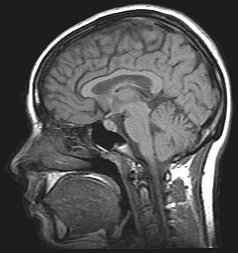
\includegraphics{brain.jpg}
\caption{}
\end{figure}

    The question we want to answer is:

\textbf{\emph{Are a person's brain size and body size predictive of his
or her intelligence?}}

Interested in answering the above research question, some researchers
(Willerman, et al, 1991) collected the following data (iqsize.txt) on a
sample of n = 38 college students.

\begin{itemize}
\tightlist
\item
  Response (y): Performance IQ scores (PIQ) from the revised Wechsler
  Adult Intelligence Scale. This variable served as the investigator's
  measure of the individual's intelligence.
\item
  Potential predictor (x1): Brain size based on the count obtained from
  MRI scans (given as count/10,000).
\item
  Potential predictor (x2): Height in inches.
\item
  Potential predictor (x3): Weight in pounds.
\end{itemize}

Source: https://onlinecourses.science.psu.edu/stat501/node/284/

    \begin{Verbatim}[commandchars=\\\{\}]
{\color{incolor}In [{\color{incolor}5}]:} \PY{n}{data} \PY{o}{=} \PY{n}{pd}\PY{o}{.}\PY{n}{read\PYZus{}csv}\PY{p}{(}\PY{l+s+s2}{\PYZdq{}}\PY{l+s+s2}{iqsize.txt}\PY{l+s+s2}{\PYZdq{}}\PY{p}{,} \PY{n}{sep} \PY{o}{=} \PY{l+s+s1}{\PYZsq{}}\PY{l+s+se}{\PYZbs{}t}\PY{l+s+s1}{\PYZsq{}}\PY{p}{)}
\end{Verbatim}


    \begin{Verbatim}[commandchars=\\\{\}]
{\color{incolor}In [{\color{incolor}6}]:} \PY{n}{data}\PY{o}{.}\PY{n}{head}\PY{p}{(}\PY{p}{)}
\end{Verbatim}


\begin{Verbatim}[commandchars=\\\{\}]
{\color{outcolor}Out[{\color{outcolor}6}]:}    PIQ   Brain  Height  Weight
        0  124   81.69    64.5     118
        1  150  103.84    73.3     143
        2  128   96.54    68.8     172
        3  134   95.15    65.0     147
        4  110   92.88    69.0     146
\end{Verbatim}
            
    \begin{Verbatim}[commandchars=\\\{\}]
{\color{incolor}In [{\color{incolor}7}]:} \PY{n}{data}\PY{o}{.}\PY{n}{size}
\end{Verbatim}


\begin{Verbatim}[commandchars=\\\{\}]
{\color{outcolor}Out[{\color{outcolor}7}]:} 152
\end{Verbatim}
            
    \section{Some Data Analysis}\label{some-data-analysis}

    \begin{Verbatim}[commandchars=\\\{\}]
{\color{incolor}In [{\color{incolor}11}]:} \PY{n}{scatter\PYZus{}matrix}\PY{p}{(}\PY{n}{data}\PY{p}{,} \PY{n}{alpha} \PY{o}{=} \PY{l+m+mf}{0.5}\PY{p}{,} \PY{n}{figsize} \PY{o}{=} \PY{p}{(}\PY{l+m+mi}{12}\PY{p}{,} \PY{l+m+mi}{12}\PY{p}{)}\PY{p}{,} \PY{n}{diagonal} \PY{o}{=} \PY{l+s+s1}{\PYZsq{}}\PY{l+s+s1}{kde}\PY{l+s+s1}{\PYZsq{}}\PY{p}{)}
\end{Verbatim}


\begin{Verbatim}[commandchars=\\\{\}]
{\color{outcolor}Out[{\color{outcolor}11}]:} array([[<matplotlib.axes.\_subplots.AxesSubplot object at 0x000001BD9EEE5320>,
                 <matplotlib.axes.\_subplots.AxesSubplot object at 0x000001BD9F2C43C8>,
                 <matplotlib.axes.\_subplots.AxesSubplot object at 0x000001BD9F2FE3C8>,
                 <matplotlib.axes.\_subplots.AxesSubplot object at 0x000001BD9F31D6A0>],
                [<matplotlib.axes.\_subplots.AxesSubplot object at 0x000001BD9F3733C8>,
                 <matplotlib.axes.\_subplots.AxesSubplot object at 0x000001BD9F373400>,
                 <matplotlib.axes.\_subplots.AxesSubplot object at 0x000001BD9F3D3DD8>,
                 <matplotlib.axes.\_subplots.AxesSubplot object at 0x000001BD9F4192E8>],
                [<matplotlib.axes.\_subplots.AxesSubplot object at 0x000001BD9F450828>,
                 <matplotlib.axes.\_subplots.AxesSubplot object at 0x000001BD9F3AC128>,
                 <matplotlib.axes.\_subplots.AxesSubplot object at 0x000001BD9F4B6DD8>,
                 <matplotlib.axes.\_subplots.AxesSubplot object at 0x000001BD9F4EBE48>],
                [<matplotlib.axes.\_subplots.AxesSubplot object at 0x000001BD9F528E48>,
                 <matplotlib.axes.\_subplots.AxesSubplot object at 0x000001BD9F563E48>,
                 <matplotlib.axes.\_subplots.AxesSubplot object at 0x000001BD9EEFA400>,
                 <matplotlib.axes.\_subplots.AxesSubplot object at 0x000001BD9F59DC88>]], dtype=object)
\end{Verbatim}
            
    \begin{center}
    \adjustimage{max size={0.9\linewidth}{0.9\paperheight}}{output_148_1.png}
    \end{center}
    { \hspace*{\fill} \\}
    
    \section{Linear Regression}\label{linear-regression}

    So basically for each observation we will try to find the best
parameters \({\bf p} = (p_0, p_1, p_2, p_3)\) that minimize the MSE for
our data

\[
\hat y_i=p_0+p_1x_{i1}+p_2x_{i2}+p_3x_{i3}
\]

The MSE is the Mean Squared Error and it looks like

\[
MSE = \frac{1}{N}\sum_i (y_i - \hat y_i)^2
\]

where \(y_i\) represent the \(i^{th}\) observation and \(\hat y_i\)
represents the \(i^{th}\) prediction. The sum is over all observations,
and \(N\) is the number of observations we have at our disposal. In our
case \(N=152\).

    \subsection{Implementation}\label{implementation}

    Let's now build our matrices. Let's start with \(Y\)

    \begin{Verbatim}[commandchars=\\\{\}]
{\color{incolor}In [{\color{incolor}38}]:} \PY{n}{Y} \PY{o}{=} \PY{n}{data}\PY{p}{[}\PY{l+s+s2}{\PYZdq{}}\PY{l+s+s2}{PIQ}\PY{l+s+s2}{\PYZdq{}}\PY{p}{]}
\end{Verbatim}


    \begin{Verbatim}[commandchars=\\\{\}]
{\color{incolor}In [{\color{incolor}39}]:} \PY{n}{Y}\PY{o}{.}\PY{n}{head}\PY{p}{(}\PY{p}{)}
\end{Verbatim}


\begin{Verbatim}[commandchars=\\\{\}]
{\color{outcolor}Out[{\color{outcolor}39}]:} 0    124
         1    150
         2    128
         3    134
         4    110
         Name: PIQ, dtype: int64
\end{Verbatim}
            
    \begin{Verbatim}[commandchars=\\\{\}]
{\color{incolor}In [{\color{incolor}46}]:} \PY{n}{X} \PY{o}{=} \PY{n}{data}\PY{o}{.}\PY{n}{drop}\PY{p}{(}\PY{l+s+s2}{\PYZdq{}}\PY{l+s+s2}{PIQ}\PY{l+s+s2}{\PYZdq{}}\PY{p}{,} \PY{n}{axis} \PY{o}{=} \PY{l+m+mi}{1}\PY{p}{)}
\end{Verbatim}


    \begin{Verbatim}[commandchars=\\\{\}]
{\color{incolor}In [{\color{incolor}47}]:} \PY{n}{X}\PY{o}{.}\PY{n}{head}\PY{p}{(}\PY{p}{)}
\end{Verbatim}


\begin{Verbatim}[commandchars=\\\{\}]
{\color{outcolor}Out[{\color{outcolor}47}]:}     Brain  Height  Weight
         0   81.69    64.5     118
         1  103.84    73.3     143
         2   96.54    68.8     172
         3   95.15    65.0     147
         4   92.88    69.0     146
\end{Verbatim}
            
    \begin{quote}
Remember: \texttt{.drop()} don't change the object in place.
\end{quote}

    So we have three features so our \(X\) matrix will have \(N\times 4\)
dimensions. Let's build it addint a columnd with all ones.

    \begin{Verbatim}[commandchars=\\\{\}]
{\color{incolor}In [{\color{incolor}48}]:} \PY{n}{X}\PY{p}{[}\PY{l+s+s2}{\PYZdq{}}\PY{l+s+s2}{b}\PY{l+s+s2}{\PYZdq{}}\PY{p}{]} \PY{o}{=} \PY{l+m+mi}{1}
\end{Verbatim}


    \begin{Verbatim}[commandchars=\\\{\}]
{\color{incolor}In [{\color{incolor}49}]:} \PY{n}{X}\PY{o}{.}\PY{n}{head}\PY{p}{(}\PY{p}{)}
\end{Verbatim}


\begin{Verbatim}[commandchars=\\\{\}]
{\color{outcolor}Out[{\color{outcolor}49}]:}     Brain  Height  Weight  b
         0   81.69    64.5     118  1
         1  103.84    73.3     143  1
         2   96.54    68.8     172  1
         3   95.15    65.0     147  1
         4   92.88    69.0     146  1
\end{Verbatim}
            
    Let's reorder the column to have the ones at the first place. This is
not strictly necessary, you just need to know how to interpret your
output vector \(\bf p\) in the results.

    \begin{Verbatim}[commandchars=\\\{\}]
{\color{incolor}In [{\color{incolor}52}]:} \PY{n}{cols} \PY{o}{=} \PY{n}{X}\PY{o}{.}\PY{n}{columns}\PY{o}{.}\PY{n}{tolist}\PY{p}{(}\PY{p}{)}
         \PY{n}{cols} \PY{o}{=} \PY{n}{cols}\PY{p}{[}\PY{o}{\PYZhy{}}\PY{l+m+mi}{1}\PY{p}{:}\PY{p}{]} \PY{o}{+} \PY{n}{cols}\PY{p}{[}\PY{p}{:}\PY{o}{\PYZhy{}}\PY{l+m+mi}{1}\PY{p}{]}
         \PY{n+nb}{print}\PY{p}{(}\PY{n}{cols}\PY{p}{)}
\end{Verbatim}


    \begin{Verbatim}[commandchars=\\\{\}]
['b', 'Brain', 'Height', 'Weight']

    \end{Verbatim}

    \begin{Verbatim}[commandchars=\\\{\}]
{\color{incolor}In [{\color{incolor}53}]:} \PY{n}{X} \PY{o}{=} \PY{n}{X}\PY{p}{[}\PY{n}{cols}\PY{p}{]}
\end{Verbatim}


    \begin{Verbatim}[commandchars=\\\{\}]
{\color{incolor}In [{\color{incolor}54}]:} \PY{n}{X}\PY{o}{.}\PY{n}{head}\PY{p}{(}\PY{p}{)}
\end{Verbatim}


\begin{Verbatim}[commandchars=\\\{\}]
{\color{outcolor}Out[{\color{outcolor}54}]:}    b   Brain  Height  Weight
         0  1   81.69    64.5     118
         1  1  103.84    73.3     143
         2  1   96.54    68.8     172
         3  1   95.15    65.0     147
         4  1   92.88    69.0     146
\end{Verbatim}
            
    Now we have the matrices we need and we can calculate

\[
{\bf p} =(X^TX)^{-1} X^T Y
\]

    \begin{Verbatim}[commandchars=\\\{\}]
{\color{incolor}In [{\color{incolor}57}]:} \PY{n}{part1} \PY{o}{=} \PY{n}{np}\PY{o}{.}\PY{n}{linalg}\PY{o}{.}\PY{n}{inv}\PY{p}{(}\PY{n}{np}\PY{o}{.}\PY{n}{matmul}\PY{p}{(}\PY{n}{X}\PY{o}{.}\PY{n}{transpose}\PY{p}{(}\PY{p}{)} \PY{p}{,} \PY{n}{X}\PY{p}{)}\PY{p}{)}
         \PY{n}{part2} \PY{o}{=} \PY{n}{np}\PY{o}{.}\PY{n}{matmul}\PY{p}{(}\PY{n}{X}\PY{o}{.}\PY{n}{transpose}\PY{p}{(}\PY{p}{)}\PY{p}{,} \PY{n}{Y}\PY{p}{)}
         
         \PY{n}{p} \PY{o}{=} \PY{n}{np}\PY{o}{.}\PY{n}{matmul}\PY{p}{(}\PY{n}{part1}\PY{p}{,} \PY{n}{part2}\PY{p}{)}
\end{Verbatim}


    \begin{Verbatim}[commandchars=\\\{\}]
{\color{incolor}In [{\color{incolor}58}]:} \PY{n+nb}{print}\PY{p}{(}\PY{n}{p}\PY{p}{)}
\end{Verbatim}


    \begin{Verbatim}[commandchars=\\\{\}]
[  1.11353608e+02   2.06036680e+00  -2.73192916e+00   5.59937127e-04]

    \end{Verbatim}

    Our prediction would look like this

    \begin{Verbatim}[commandchars=\\\{\}]
{\color{incolor}In [{\color{incolor}61}]:} \PY{n}{Yhat} \PY{o}{=} \PY{n}{np}\PY{o}{.}\PY{n}{matmul}\PY{p}{(}\PY{n}{X}\PY{p}{,} \PY{n}{p}\PY{p}{)}
\end{Verbatim}


    \begin{Verbatim}[commandchars=\\\{\}]
{\color{incolor}In [{\color{incolor}70}]:} \PY{n}{plt}\PY{o}{.}\PY{n}{rc}\PY{p}{(}\PY{l+s+s1}{\PYZsq{}}\PY{l+s+s1}{font}\PY{l+s+s1}{\PYZsq{}}\PY{p}{,} \PY{n}{family}\PY{o}{=}\PY{l+s+s1}{\PYZsq{}}\PY{l+s+s1}{arial}\PY{l+s+s1}{\PYZsq{}}\PY{p}{)}
         \PY{n}{plt}\PY{o}{.}\PY{n}{rc}\PY{p}{(}\PY{l+s+s1}{\PYZsq{}}\PY{l+s+s1}{xtick}\PY{l+s+s1}{\PYZsq{}}\PY{p}{,} \PY{n}{labelsize}\PY{o}{=}\PY{l+s+s1}{\PYZsq{}}\PY{l+s+s1}{x\PYZhy{}small}\PY{l+s+s1}{\PYZsq{}}\PY{p}{)}
         \PY{n}{plt}\PY{o}{.}\PY{n}{rc}\PY{p}{(}\PY{l+s+s1}{\PYZsq{}}\PY{l+s+s1}{ytick}\PY{l+s+s1}{\PYZsq{}}\PY{p}{,} \PY{n}{labelsize}\PY{o}{=}\PY{l+s+s1}{\PYZsq{}}\PY{l+s+s1}{x\PYZhy{}small}\PY{l+s+s1}{\PYZsq{}}\PY{p}{)}
             
         \PY{n}{plt}\PY{o}{.}\PY{n}{tight\PYZus{}layout}\PY{p}{(}\PY{p}{)}
         
         \PY{n}{fig} \PY{o}{=} \PY{n}{plt}\PY{o}{.}\PY{n}{figure}\PY{p}{(}\PY{n}{figsize}\PY{o}{=}\PY{p}{(}\PY{l+m+mi}{8}\PY{p}{,} \PY{l+m+mi}{5}\PY{p}{)}\PY{p}{)}
         \PY{n}{ax} \PY{o}{=} \PY{n}{fig}\PY{o}{.}\PY{n}{add\PYZus{}subplot}\PY{p}{(}\PY{l+m+mi}{1}\PY{p}{,} \PY{l+m+mi}{1}\PY{p}{,} \PY{l+m+mi}{1}\PY{p}{)}
         \PY{n}{ax}\PY{o}{.}\PY{n}{scatter}\PY{p}{(}\PY{n}{Y}\PY{p}{,} \PY{n}{Yhat}\PY{p}{,} \PY{n}{lw} \PY{o}{=} \PY{l+m+mf}{0.3}\PY{p}{)}
         \PY{n}{ax}\PY{o}{.}\PY{n}{plot}\PY{p}{(}\PY{p}{[}\PY{n}{Y}\PY{o}{.}\PY{n}{min}\PY{p}{(}\PY{p}{)}\PY{p}{,} \PY{n}{Y}\PY{o}{.}\PY{n}{max}\PY{p}{(}\PY{p}{)}\PY{p}{]}\PY{p}{,} \PY{p}{[}\PY{n}{Y}\PY{o}{.}\PY{n}{min}\PY{p}{(}\PY{p}{)}\PY{p}{,} \PY{n}{Y}\PY{o}{.}\PY{n}{max}\PY{p}{(}\PY{p}{)}\PY{p}{]}\PY{p}{,} \PY{l+s+s1}{\PYZsq{}}\PY{l+s+s1}{k\PYZhy{}\PYZhy{}}\PY{l+s+s1}{\PYZsq{}}\PY{p}{,} \PY{n}{lw} \PY{o}{=} \PY{l+m+mi}{3}\PY{p}{)}
         \PY{n}{ax}\PY{o}{.}\PY{n}{set\PYZus{}xlabel}\PY{p}{(}\PY{l+s+s1}{\PYZsq{}}\PY{l+s+s1}{Measured Target Value}\PY{l+s+s1}{\PYZsq{}}\PY{p}{)}
         \PY{n}{ax}\PY{o}{.}\PY{n}{set\PYZus{}ylabel}\PY{p}{(}\PY{l+s+s1}{\PYZsq{}}\PY{l+s+s1}{Predicted Target Value}\PY{l+s+s1}{\PYZsq{}}\PY{p}{)}
\end{Verbatim}


\begin{Verbatim}[commandchars=\\\{\}]
{\color{outcolor}Out[{\color{outcolor}70}]:} Text(0,0.5,'Predicted Target Value')
\end{Verbatim}
            
    
    \begin{verbatim}
<matplotlib.figure.Figure at 0x210a33dcc18>
    \end{verbatim}

    
    \begin{center}
    \adjustimage{max size={0.9\linewidth}{0.9\paperheight}}{output_170_2.png}
    \end{center}
    { \hspace*{\fill} \\}
    
    \subsection{Example of linear regression in
sklearn}\label{example-of-linear-regression-in-sklearn}

    \begin{Verbatim}[commandchars=\\\{\}]
{\color{incolor}In [{\color{incolor}78}]:} \PY{k+kn}{from} \PY{n+nn}{sklearn} \PY{k}{import} \PY{n}{datasets}\PY{p}{,} \PY{n}{linear\PYZus{}model}
         \PY{k+kn}{from} \PY{n+nn}{sklearn}\PY{n+nn}{.}\PY{n+nn}{metrics} \PY{k}{import} \PY{n}{mean\PYZus{}squared\PYZus{}error}\PY{p}{,} \PY{n}{r2\PYZus{}score}
         
         \PY{n}{regr} \PY{o}{=} \PY{n}{linear\PYZus{}model}\PY{o}{.}\PY{n}{LinearRegression}\PY{p}{(}\PY{p}{)}
         \PY{n}{regr}\PY{o}{.}\PY{n}{fit}\PY{p}{(}\PY{n}{X}\PY{o}{.}\PY{n}{drop}\PY{p}{(}\PY{l+s+s1}{\PYZsq{}}\PY{l+s+s1}{b}\PY{l+s+s1}{\PYZsq{}}\PY{p}{,} \PY{n}{axis} \PY{o}{=} \PY{l+m+mi}{1}\PY{p}{)}\PY{p}{,} \PY{n}{Y}\PY{p}{)}
\end{Verbatim}


\begin{Verbatim}[commandchars=\\\{\}]
{\color{outcolor}Out[{\color{outcolor}78}]:} LinearRegression(copy\_X=True, fit\_intercept=True, n\_jobs=1, normalize=False)
\end{Verbatim}
            
    \begin{Verbatim}[commandchars=\\\{\}]
{\color{incolor}In [{\color{incolor}79}]:} \PY{n}{y\PYZus{}pred} \PY{o}{=} \PY{n}{regr}\PY{o}{.}\PY{n}{predict}\PY{p}{(}\PY{n}{X}\PY{o}{.}\PY{n}{drop}\PY{p}{(}\PY{l+s+s1}{\PYZsq{}}\PY{l+s+s1}{b}\PY{l+s+s1}{\PYZsq{}}\PY{p}{,} \PY{n}{axis} \PY{o}{=} \PY{l+m+mi}{1}\PY{p}{)}\PY{p}{)}
\end{Verbatim}


    \begin{Verbatim}[commandchars=\\\{\}]
{\color{incolor}In [{\color{incolor}83}]:} \PY{n+nb}{print}\PY{p}{(}\PY{l+s+s1}{\PYZsq{}}\PY{l+s+s1}{Coefficients: }\PY{l+s+s1}{\PYZsq{}}\PY{p}{,} \PY{n}{regr}\PY{o}{.}\PY{n}{coef\PYZus{}}\PY{p}{)}
         \PY{n+nb}{print}\PY{p}{(}\PY{l+s+s1}{\PYZsq{}}\PY{l+s+s1}{Intercept: }\PY{l+s+s1}{\PYZsq{}}\PY{p}{,} \PY{n}{regr}\PY{o}{.}\PY{n}{intercept\PYZus{}}\PY{p}{)}
\end{Verbatim}


    \begin{Verbatim}[commandchars=\\\{\}]
Coefficients:  [  2.06036680e+00  -2.73192916e+00   5.59937127e-04]
Intercept:  111.353608292

    \end{Verbatim}

    Let's compare the parameters with what we got with our matrix solution

    \begin{Verbatim}[commandchars=\\\{\}]
{\color{incolor}In [{\color{incolor}87}]:} \PY{n+nb}{print}\PY{p}{(}\PY{l+s+s1}{\PYZsq{}}\PY{l+s+s1}{Coefficients from the matrix model: }\PY{l+s+s1}{\PYZsq{}}\PY{p}{,} \PY{n}{p}\PY{p}{[}\PY{l+m+mi}{1}\PY{p}{:}\PY{l+m+mi}{4}\PY{p}{]}\PY{p}{)}
         \PY{n+nb}{print}\PY{p}{(}\PY{l+s+s1}{\PYZsq{}}\PY{l+s+s1}{Coefficients obtained with sklearn: }\PY{l+s+s1}{\PYZsq{}}\PY{p}{,} \PY{n}{regr}\PY{o}{.}\PY{n}{coef\PYZus{}}\PY{p}{)}
         \PY{n+nb}{print}\PY{p}{(}\PY{l+s+s1}{\PYZsq{}}\PY{l+s+s1}{Intercept obtained with sklearn: }\PY{l+s+s1}{\PYZsq{}}\PY{p}{,} \PY{n}{p}\PY{p}{[}\PY{l+m+mi}{0}\PY{p}{]}\PY{p}{)}
         \PY{n+nb}{print}\PY{p}{(}\PY{l+s+s1}{\PYZsq{}}\PY{l+s+s1}{Intercept obtained with sklearn: }\PY{l+s+s1}{\PYZsq{}}\PY{p}{,} \PY{n}{regr}\PY{o}{.}\PY{n}{intercept\PYZus{}}\PY{p}{)}
\end{Verbatim}


    \begin{Verbatim}[commandchars=\\\{\}]
Coefficients from the matrix model:  [  2.06036680e+00  -2.73192916e+00   5.59937127e-04]
Coefficients obtained with sklearn:  [  2.06036680e+00  -2.73192916e+00   5.59937127e-04]
Intercept obtained with sklearn:  111.353608292
Intercept obtained with sklearn:  111.353608292

    \end{Verbatim}

    As you will notice they are the same (as they should be).

    \begin{Verbatim}[commandchars=\\\{\}]
{\color{incolor}In [{\color{incolor}82}]:} \PY{n}{plt}\PY{o}{.}\PY{n}{rc}\PY{p}{(}\PY{l+s+s1}{\PYZsq{}}\PY{l+s+s1}{font}\PY{l+s+s1}{\PYZsq{}}\PY{p}{,} \PY{n}{family}\PY{o}{=}\PY{l+s+s1}{\PYZsq{}}\PY{l+s+s1}{arial}\PY{l+s+s1}{\PYZsq{}}\PY{p}{)}
         \PY{n}{plt}\PY{o}{.}\PY{n}{rc}\PY{p}{(}\PY{l+s+s1}{\PYZsq{}}\PY{l+s+s1}{xtick}\PY{l+s+s1}{\PYZsq{}}\PY{p}{,} \PY{n}{labelsize}\PY{o}{=}\PY{l+s+s1}{\PYZsq{}}\PY{l+s+s1}{x\PYZhy{}small}\PY{l+s+s1}{\PYZsq{}}\PY{p}{)}
         \PY{n}{plt}\PY{o}{.}\PY{n}{rc}\PY{p}{(}\PY{l+s+s1}{\PYZsq{}}\PY{l+s+s1}{ytick}\PY{l+s+s1}{\PYZsq{}}\PY{p}{,} \PY{n}{labelsize}\PY{o}{=}\PY{l+s+s1}{\PYZsq{}}\PY{l+s+s1}{x\PYZhy{}small}\PY{l+s+s1}{\PYZsq{}}\PY{p}{)}
             
         \PY{n}{plt}\PY{o}{.}\PY{n}{tight\PYZus{}layout}\PY{p}{(}\PY{p}{)}
         
         \PY{n}{fig} \PY{o}{=} \PY{n}{plt}\PY{o}{.}\PY{n}{figure}\PY{p}{(}\PY{n}{figsize}\PY{o}{=}\PY{p}{(}\PY{l+m+mi}{8}\PY{p}{,} \PY{l+m+mi}{5}\PY{p}{)}\PY{p}{)}
         \PY{n}{ax} \PY{o}{=} \PY{n}{fig}\PY{o}{.}\PY{n}{add\PYZus{}subplot}\PY{p}{(}\PY{l+m+mi}{1}\PY{p}{,} \PY{l+m+mi}{1}\PY{p}{,} \PY{l+m+mi}{1}\PY{p}{)}
         \PY{n}{ax}\PY{o}{.}\PY{n}{scatter}\PY{p}{(}\PY{n}{Y}\PY{p}{,} \PY{n}{y\PYZus{}pred}\PY{p}{,} \PY{n}{lw} \PY{o}{=} \PY{l+m+mf}{0.3}\PY{p}{)}
         \PY{n}{ax}\PY{o}{.}\PY{n}{plot}\PY{p}{(}\PY{p}{[}\PY{n}{Y}\PY{o}{.}\PY{n}{min}\PY{p}{(}\PY{p}{)}\PY{p}{,} \PY{n}{Y}\PY{o}{.}\PY{n}{max}\PY{p}{(}\PY{p}{)}\PY{p}{]}\PY{p}{,} \PY{p}{[}\PY{n}{Y}\PY{o}{.}\PY{n}{min}\PY{p}{(}\PY{p}{)}\PY{p}{,} \PY{n}{Y}\PY{o}{.}\PY{n}{max}\PY{p}{(}\PY{p}{)}\PY{p}{]}\PY{p}{,} \PY{l+s+s1}{\PYZsq{}}\PY{l+s+s1}{k\PYZhy{}\PYZhy{}}\PY{l+s+s1}{\PYZsq{}}\PY{p}{,} \PY{n}{lw} \PY{o}{=} \PY{l+m+mi}{3}\PY{p}{)}
         \PY{n}{ax}\PY{o}{.}\PY{n}{set\PYZus{}xlabel}\PY{p}{(}\PY{l+s+s1}{\PYZsq{}}\PY{l+s+s1}{Measured Target Value}\PY{l+s+s1}{\PYZsq{}}\PY{p}{)}
         \PY{n}{ax}\PY{o}{.}\PY{n}{set\PYZus{}ylabel}\PY{p}{(}\PY{l+s+s1}{\PYZsq{}}\PY{l+s+s1}{Predicted Target Value}\PY{l+s+s1}{\PYZsq{}}\PY{p}{)}
\end{Verbatim}


\begin{Verbatim}[commandchars=\\\{\}]
{\color{outcolor}Out[{\color{outcolor}82}]:} Text(0,0.5,'Predicted Target Value')
\end{Verbatim}
            
    
    \begin{verbatim}
<matplotlib.figure.Figure at 0x210a53f1c50>
    \end{verbatim}

    
    \begin{center}
    \adjustimage{max size={0.9\linewidth}{0.9\paperheight}}{output_178_2.png}
    \end{center}
    { \hspace*{\fill} \\}
    
    \subsection{Exercise 6}\label{exercise-6}

    Source:
https://www.cs.toronto.edu/\textasciitilde{}delve/data/boston/bostonDetail.html

    Apply the same methods (linear regression) to a the boston housing
dataset. This dataset contains information collected by the U.S Census
Service concerning housing in the area of Boston Mass. It was obtained
from the StatLib archive (http://lib.stat.cmu.edu/datasets/boston), and
has been used extensively throughout the literature to benchmark
algorithms. However, these comparisons were primarily done outside of
Delve and are thus somewhat suspect. The dataset is small in size with
only 506 cases.

Variables There are 14 attributes in each case of the dataset. They are:
- CRIM - per capita crime rate by town - ZN - proportion of residential
land zoned for lots over 25,000 sq.ft. - INDUS - proportion of
non-retail business acres per town. - CHAS - Charles River dummy
variable (1 if tract bounds river; 0 otherwise) - NOX - nitric oxides
concentration (parts per 10 million) - RM - average number of rooms per
dwelling - AGE - proportion of owner-occupied units built prior to 1940
- DIS - weighted distances to five Boston employment centres - RAD -
index of accessibility to radial highways - TAX - full-value
property-tax rate per \$10,000 - PTRATIO - pupil-teacher ratio by town -
B - 1000(Bk - 0.63)\^{}2 where Bk is the proportion of blacks by town -
LSTAT - percentage lower status of the population - MEDV - Median value
of owner-occupied homes in \$1000's

Our target variable (what we want do predict) is the MEDV variable.

At the end plot the predicted values from your model vs. the one given
in the dataset.

    To make your life easier you can use the following to load your dataset
(you need internet)

    \begin{Verbatim}[commandchars=\\\{\}]
{\color{incolor}In [{\color{incolor}21}]:} \PY{k+kn}{from} \PY{n+nn}{sklearn}\PY{n+nn}{.}\PY{n+nn}{datasets} \PY{k}{import} \PY{n}{load\PYZus{}boston}
         \PY{n}{X}\PY{p}{,}\PY{n}{Y} \PY{o}{=} \PY{n}{load\PYZus{}boston}\PY{p}{(}\PY{n}{return\PYZus{}X\PYZus{}y} \PY{o}{=} \PY{k+kc}{True}\PY{p}{)}
\end{Verbatim}


    \begin{Verbatim}[commandchars=\\\{\}]
{\color{incolor}In [{\color{incolor}23}]:} \PY{n}{X}\PY{o}{.}\PY{n}{shape}
\end{Verbatim}


\begin{Verbatim}[commandchars=\\\{\}]
{\color{outcolor}Out[{\color{outcolor}23}]:} (506, 13)
\end{Verbatim}
            
    As expected we have \(506\) observations and \(13\) features.

    \begin{Verbatim}[commandchars=\\\{\}]
{\color{incolor}In [{\color{incolor}24}]:} \PY{n}{Y}\PY{o}{.}\PY{n}{shape}
\end{Verbatim}


\begin{Verbatim}[commandchars=\\\{\}]
{\color{outcolor}Out[{\color{outcolor}24}]:} (506,)
\end{Verbatim}
            
    \section{Exercise 7}\label{exercise-7}

    From the previous exercise you should get a plot similar to this one

\begin{figure}
\centering
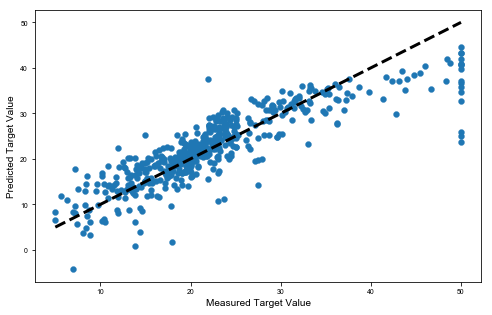
\includegraphics{boston_result.png}
\caption{}
\end{figure}

Answer why there is set of vertical point at
\texttt{"Measured\ Target\ Value\ =\ 50".}

    \section{Connection to neural networks - why do we need linear
algebra}\label{connection-to-neural-networks---why-do-we-need-linear-algebra}


    % Add a bibliography block to the postdoc
    
    
    
    \end{document}
